\section{Known Enumerative Results}

When treating the Building Game for a polyhedron as a stochastic process, we must first know what the the combinatorial configuration space is exactly. This is a computational enumeration problem, but the results of this enumeration are also of methematical interest. 

Attachment models like the Building Game have been the topic of much reserch in combinatorial mathematics. A well known example of this is the study of polyominoes. An $n$-omino is a configuration of $n$ attached squares in a $2$-dimensional latice. As seen in figure~\ref{fig:Tetris}, the classic video game tetris uses each of the seven rotationally unique tetrominoes ($n = 4$) as game pieces. The enumeration of $n$-ominoes has been extensively studied and there are many enumeration results, both explicit and asymptotic. As in our case, the general goal is to enumerate the polyominoes that are unique when acted on by some group (rotation, reflection, etc) or under certain constraints which are often topological.
\begin{figure}[ht]
  %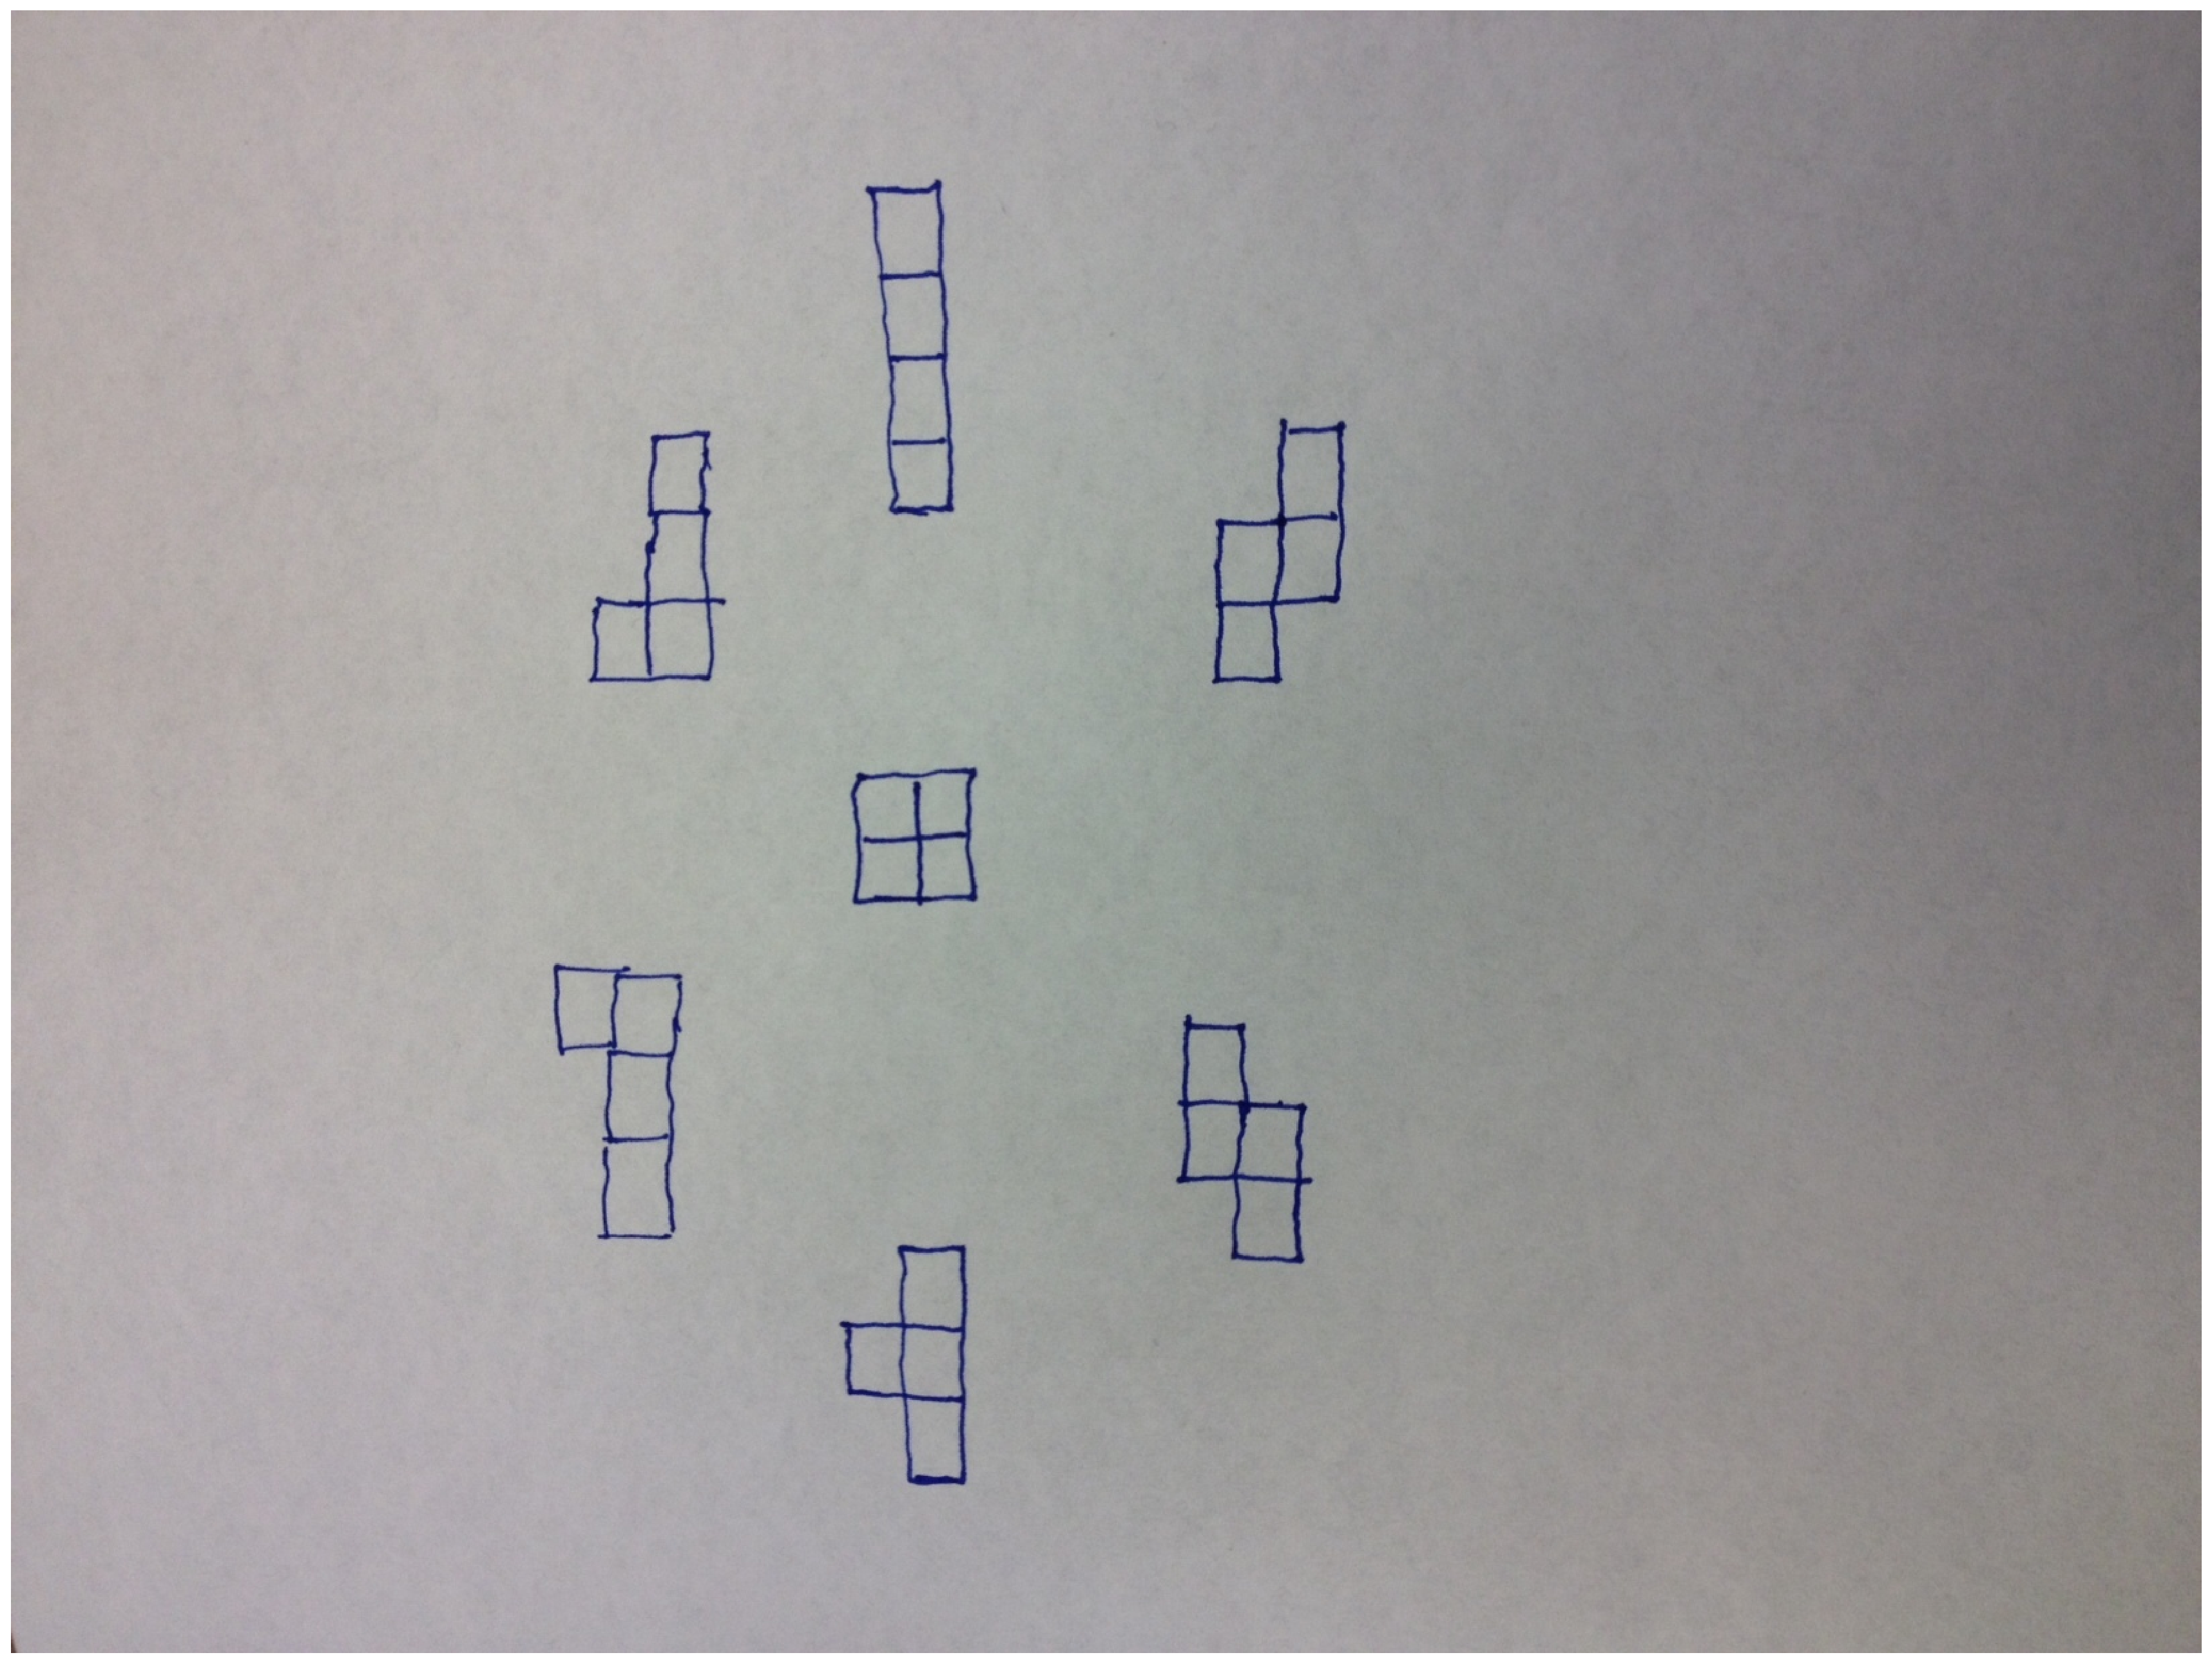
\includegraphics[scale=0.1, angle=0]{tetris.eps}
\caption{The seven tetrominoes used in Tetris.}
\label{fig:Tetris}
\end{figure}

The Building Game has a wealth of combinatorial enumeration problems to consider. Some have been addressed in the work of Zlotnick et all CITE. The original Building Game paper only considers a single pathway and thus is not conserned with enumeration of the entire combinatorial configuration space. However in Endres et al, the number of intermediates for each of the Platonic solids is computed. The entire combinatorial configuration space for the dodecahedron and icosahedron is also illustrated CITE. 

Before the work of Endres et al, David Wilson enumerated the number of intermediates composed of each number of faces for the icosahedron CITE. This computation seems to have ooccured independent of the scientific context of self-assembly as Wilson's enumerations are refered to as the ``Number of one-sided triangular n-ominoes (or triominoes) on the icosahedron.'' He also includes variants such as the ``Number of triangular n-ominoes on the icosahedron'' which enlarges the equivalence classes to identify intermediate that are reflections of each other. 

\section{New Enumerative Results}

Previous enumeration results for the Building Game have focused on the number of intermediates of the Platonic solids. We extend these results to also count the number of Building Game connections and pathways in the combinatorial configuration space. Additionally, we consider the Platonic, Archimedean, and Catalan solids classes with these results presemted in figures~\ref{tab:bgePlat}, ~\ref{tab:bgeArch} and ~\ref{tab:bgeCat} respectively. 

As we consider polyhedra with more and more faces, there is a combinatorial explosion in the number intermediates in combinatorial configuration space. This was noted in Endres et al. CITE, where the dodecahedron has $73$ intermediates and the icosahedron has $2,649$. We have enumerated the intermediates for polyhedra of up to $30$ faces in our three classes of polyhedra. The $30$-faced rhombic triacontahdron has the most intermediates of all polyhedra in our computation with $2,423,212$.



%While the 6-faced cube state space has only 8 nodes and 9 nodes, the 20-faced icosahedron state space has 2,649 nodes and 17,241 nodes and the 26-faced truncated cuboctahedron state space has 1,525,605 nodes and 17,672,377. Figure \ref{fig:bgtable} details state space sizes of all polyhedra in the Platonic, Archimedean, and Catalan solid classes of up to 26 faces. 



\begin{figure}[ht]
%\scalebox{0.6}{
%{\footnotesize
\centering
%\textbf{Building Game Enumerative Results for the Platonic Solids}
\begin{tabular}{ l | c | r | r | r}
Polyhedra Name & $|F|$ & Intermediates & Connections & Pathways \\
  \hline    
Tetrahedron                     & 4        & 4     	& 3             & 1\\
Cube                            & 6        & 8     	& 9    		& 3\\
Octahedron                      & 8        & 14    	& 21    	& 14\\
Dodecahedron                    & 12       & 73    	& 263   	& 17,696 \\
Icosahedron                     & 20       & 2,649 	& 17,241        & 57,396,146,640\\
\end{tabular}
%}
\caption{Building game enumerative results for the Platonic solids.}
\label{tab:bgePlat}
\end{figure}


\begin{figure}[ht]
%\scalebox{0.6}{
%{\footnotesize
\centering
%\textbf{Building Game Enumerative Results for the Platonic Solids}
\begin{tabular}{ l | c | r | r | r}
Polyhedra Name & $|F|$ & Intermediates & Connections & Pathways \\
  \hline    
Truncated Tetrahedron           & 8     & 28    	& 63            & 402\\
Cuboctahedron                   & 14  	& 340   	& 1,634         & 10,170,968\\
Truncated Cube                  & 14  	& 499   	& 2,729         & 101,443,338 \\
Truncated Octahedron            & 14  	& 555           & 3,069         & 68,106,377\\
Rhombicuboctahedron             & 26  	& 638,850       & 6,459,801     & 164,068,345,221,515,292,308\\
Truncated Cuboctahedron         & 26  	& 1,525,658     & 17,672,374    & 13,837,219,462,483,379,105,902\\
%Icosidodecahedron               & 32  	& ?             & ?             & ?\\
%Truncated Dodecahedron          & 32  	& ?             & ? 	        & ? \\
%Truncated Icosahedron           & 32  	& ?             & ? 	        & ?\\
\end{tabular}
%}
\caption{Building game enumerative results for the Archimedean solids.}
\label{tab:bgeArch}
\end{figure}


\begin{figure}[ht]
%\scalebox{0.6}{
%{\footnotesize
\centering
%\textbf{Building Game Enumerative Results for the Platonic Solids}
\begin{tabular}{ l | c | r | r | r}
Polyhedra Name & $|F|$ & Intermediates & Connections & Pathways \\
  \hline    
Triakis Tetrahedron             & 12  	& 98            & 318           & 38,938\\
Rhombic Dodecahedron            & 12  	& 127           & 493           & 76,936\\
Triakis Octahedron              & 24  	& 12,748        & 81,296        & 169,402,670,046,670\\
Tetrakis Hexahedron             & 24  	& 50,767        & 394,377       & 4,253,948,297,210,346\\
Deltoidal Icositetrahedron      & 24  	& 209,675       & 1,989,548     & 418,663,242,727,526,726 \\
Pentagonal Icositetrahedron     & 24  	& 345,938       & 3,544,987     & 2,828,128,000,716,774,492\\
Rhombic Triacontahedron         & 30  	& 2,423,212     & 26,823,095    & 161,598,744,916,797,017,978,128\\
\end{tabular}
%}
\caption{Building game enumerative results for the Catalan solids.}
\label{tab:bgeCat}
\end{figure}




\begin{figure}[ht]
  %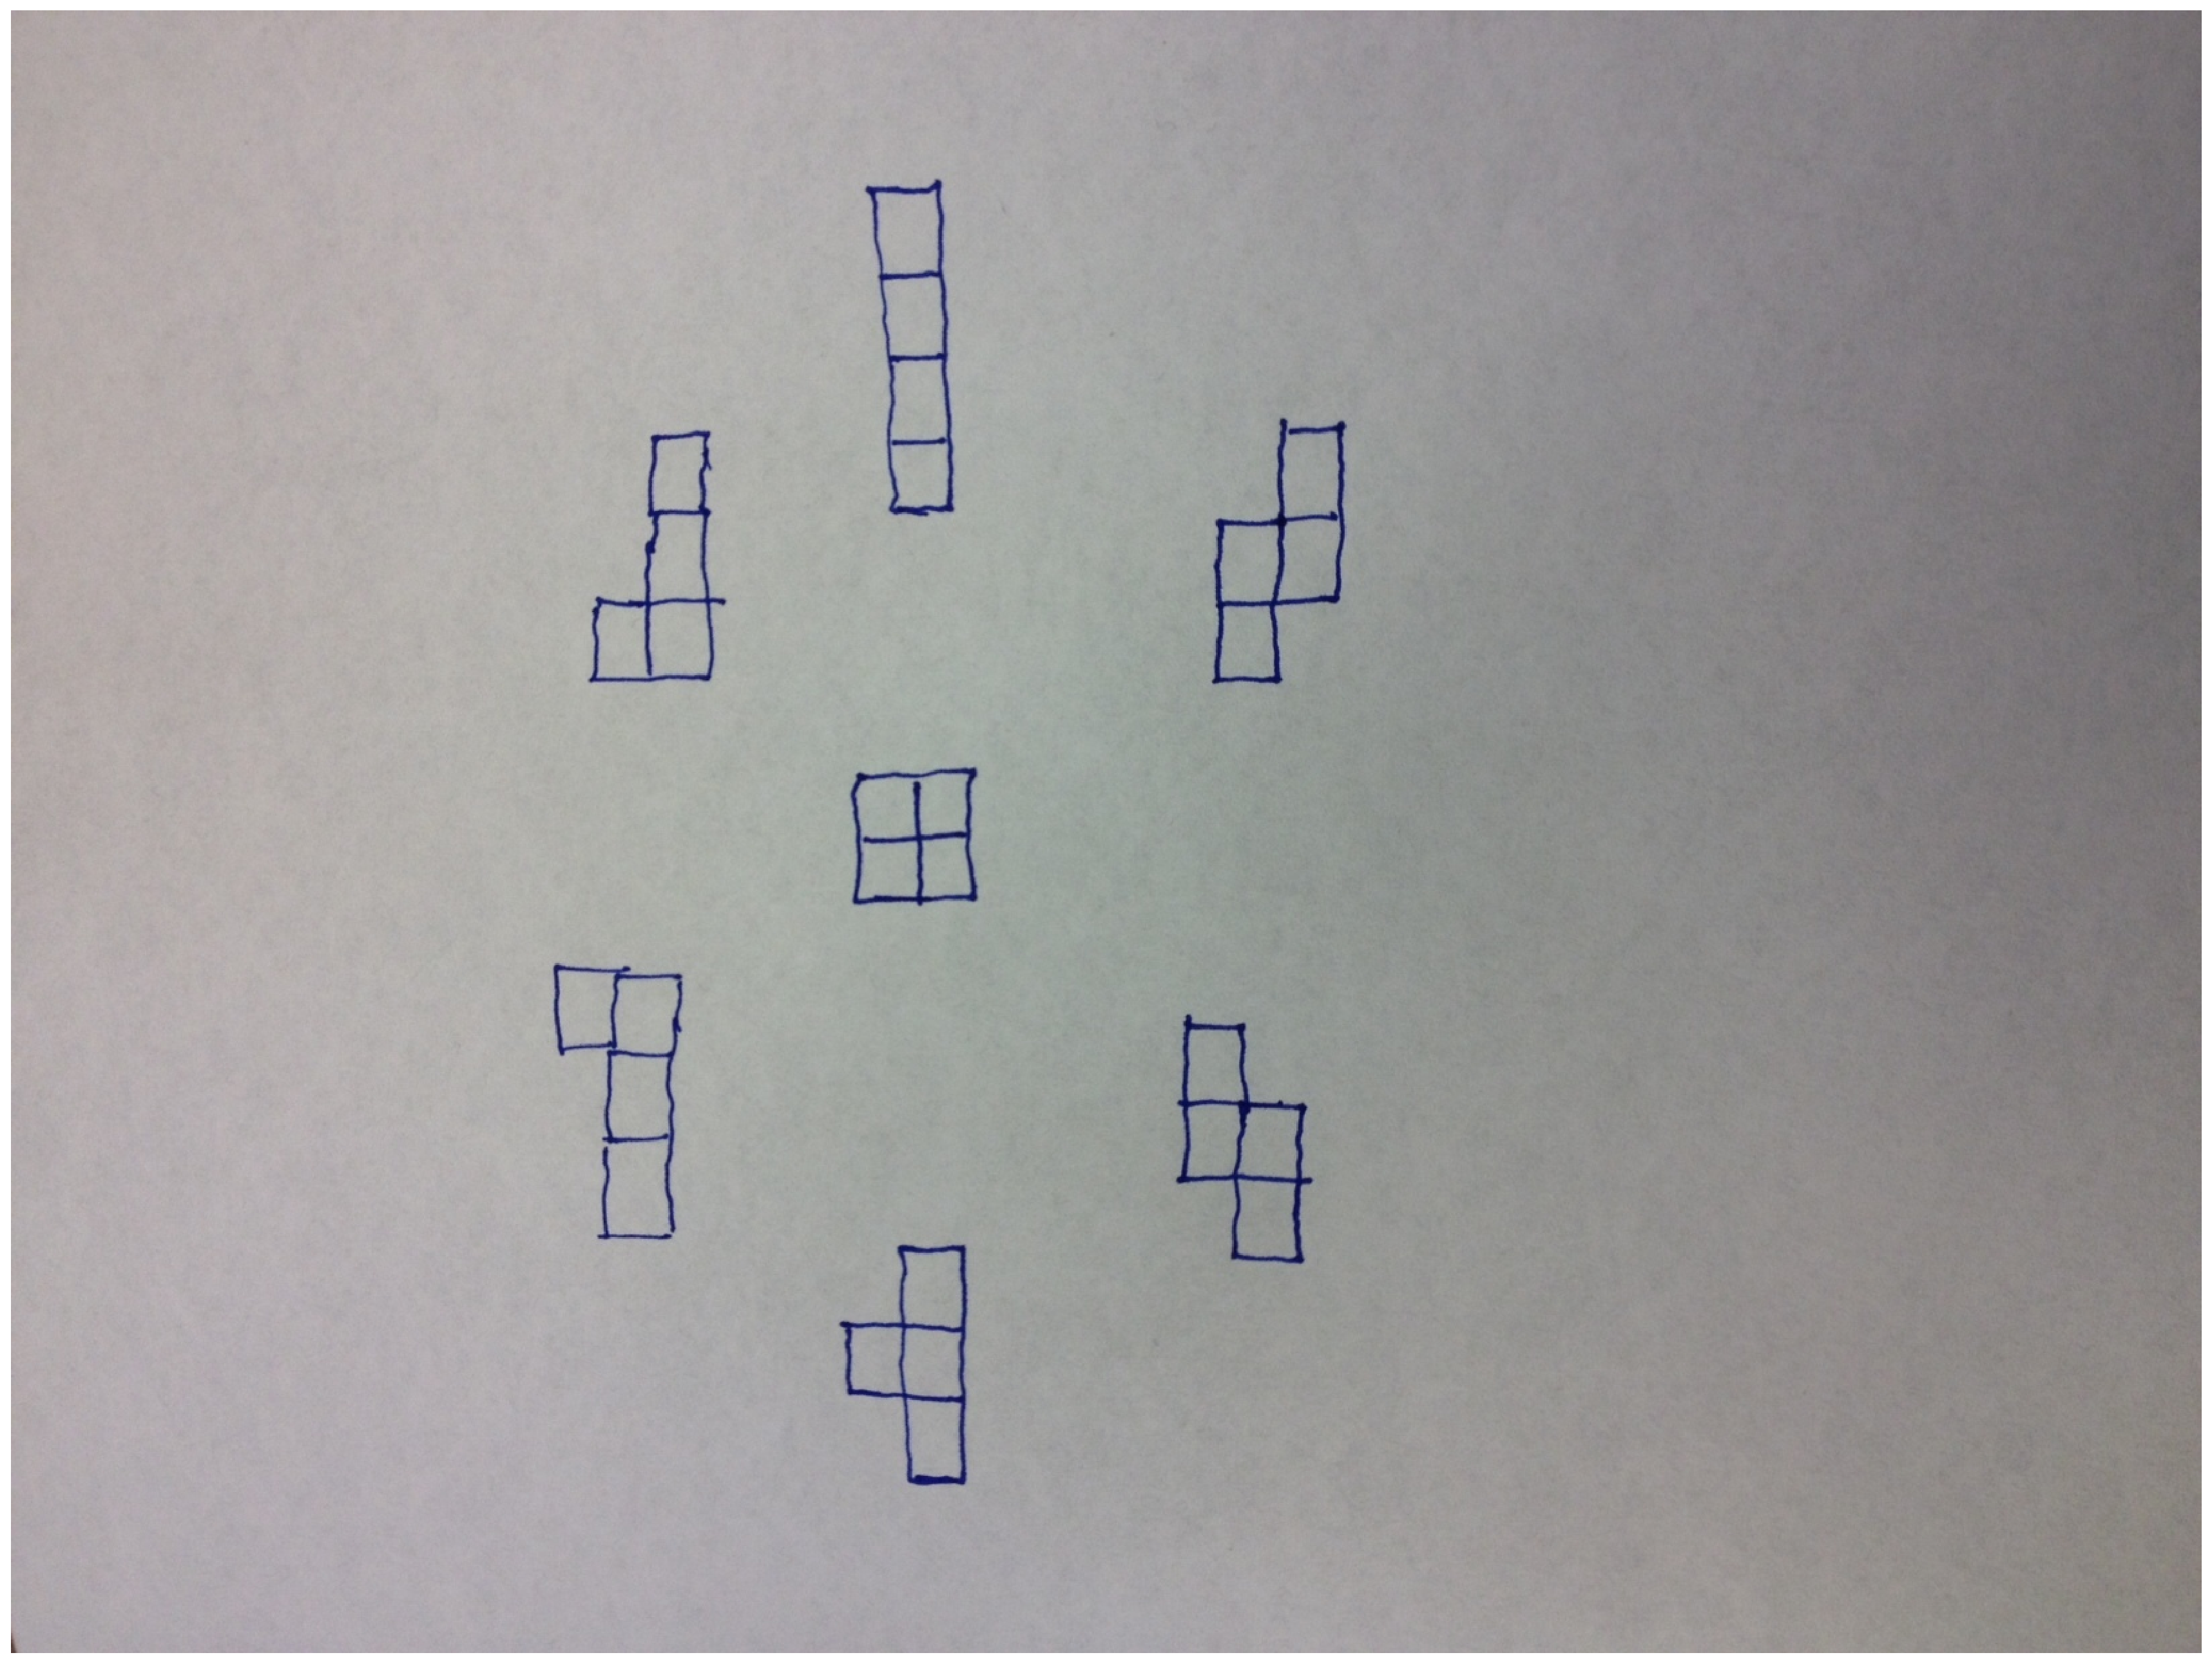
\includegraphics[scale=0.1, angle=0]{tetris.eps}
\caption{The relation between number of faces and intermediates in the Building Game combinatorial configuration space.}
\label{fig:FacInt}
\end{figure}

\begin{figure}[ht]
  %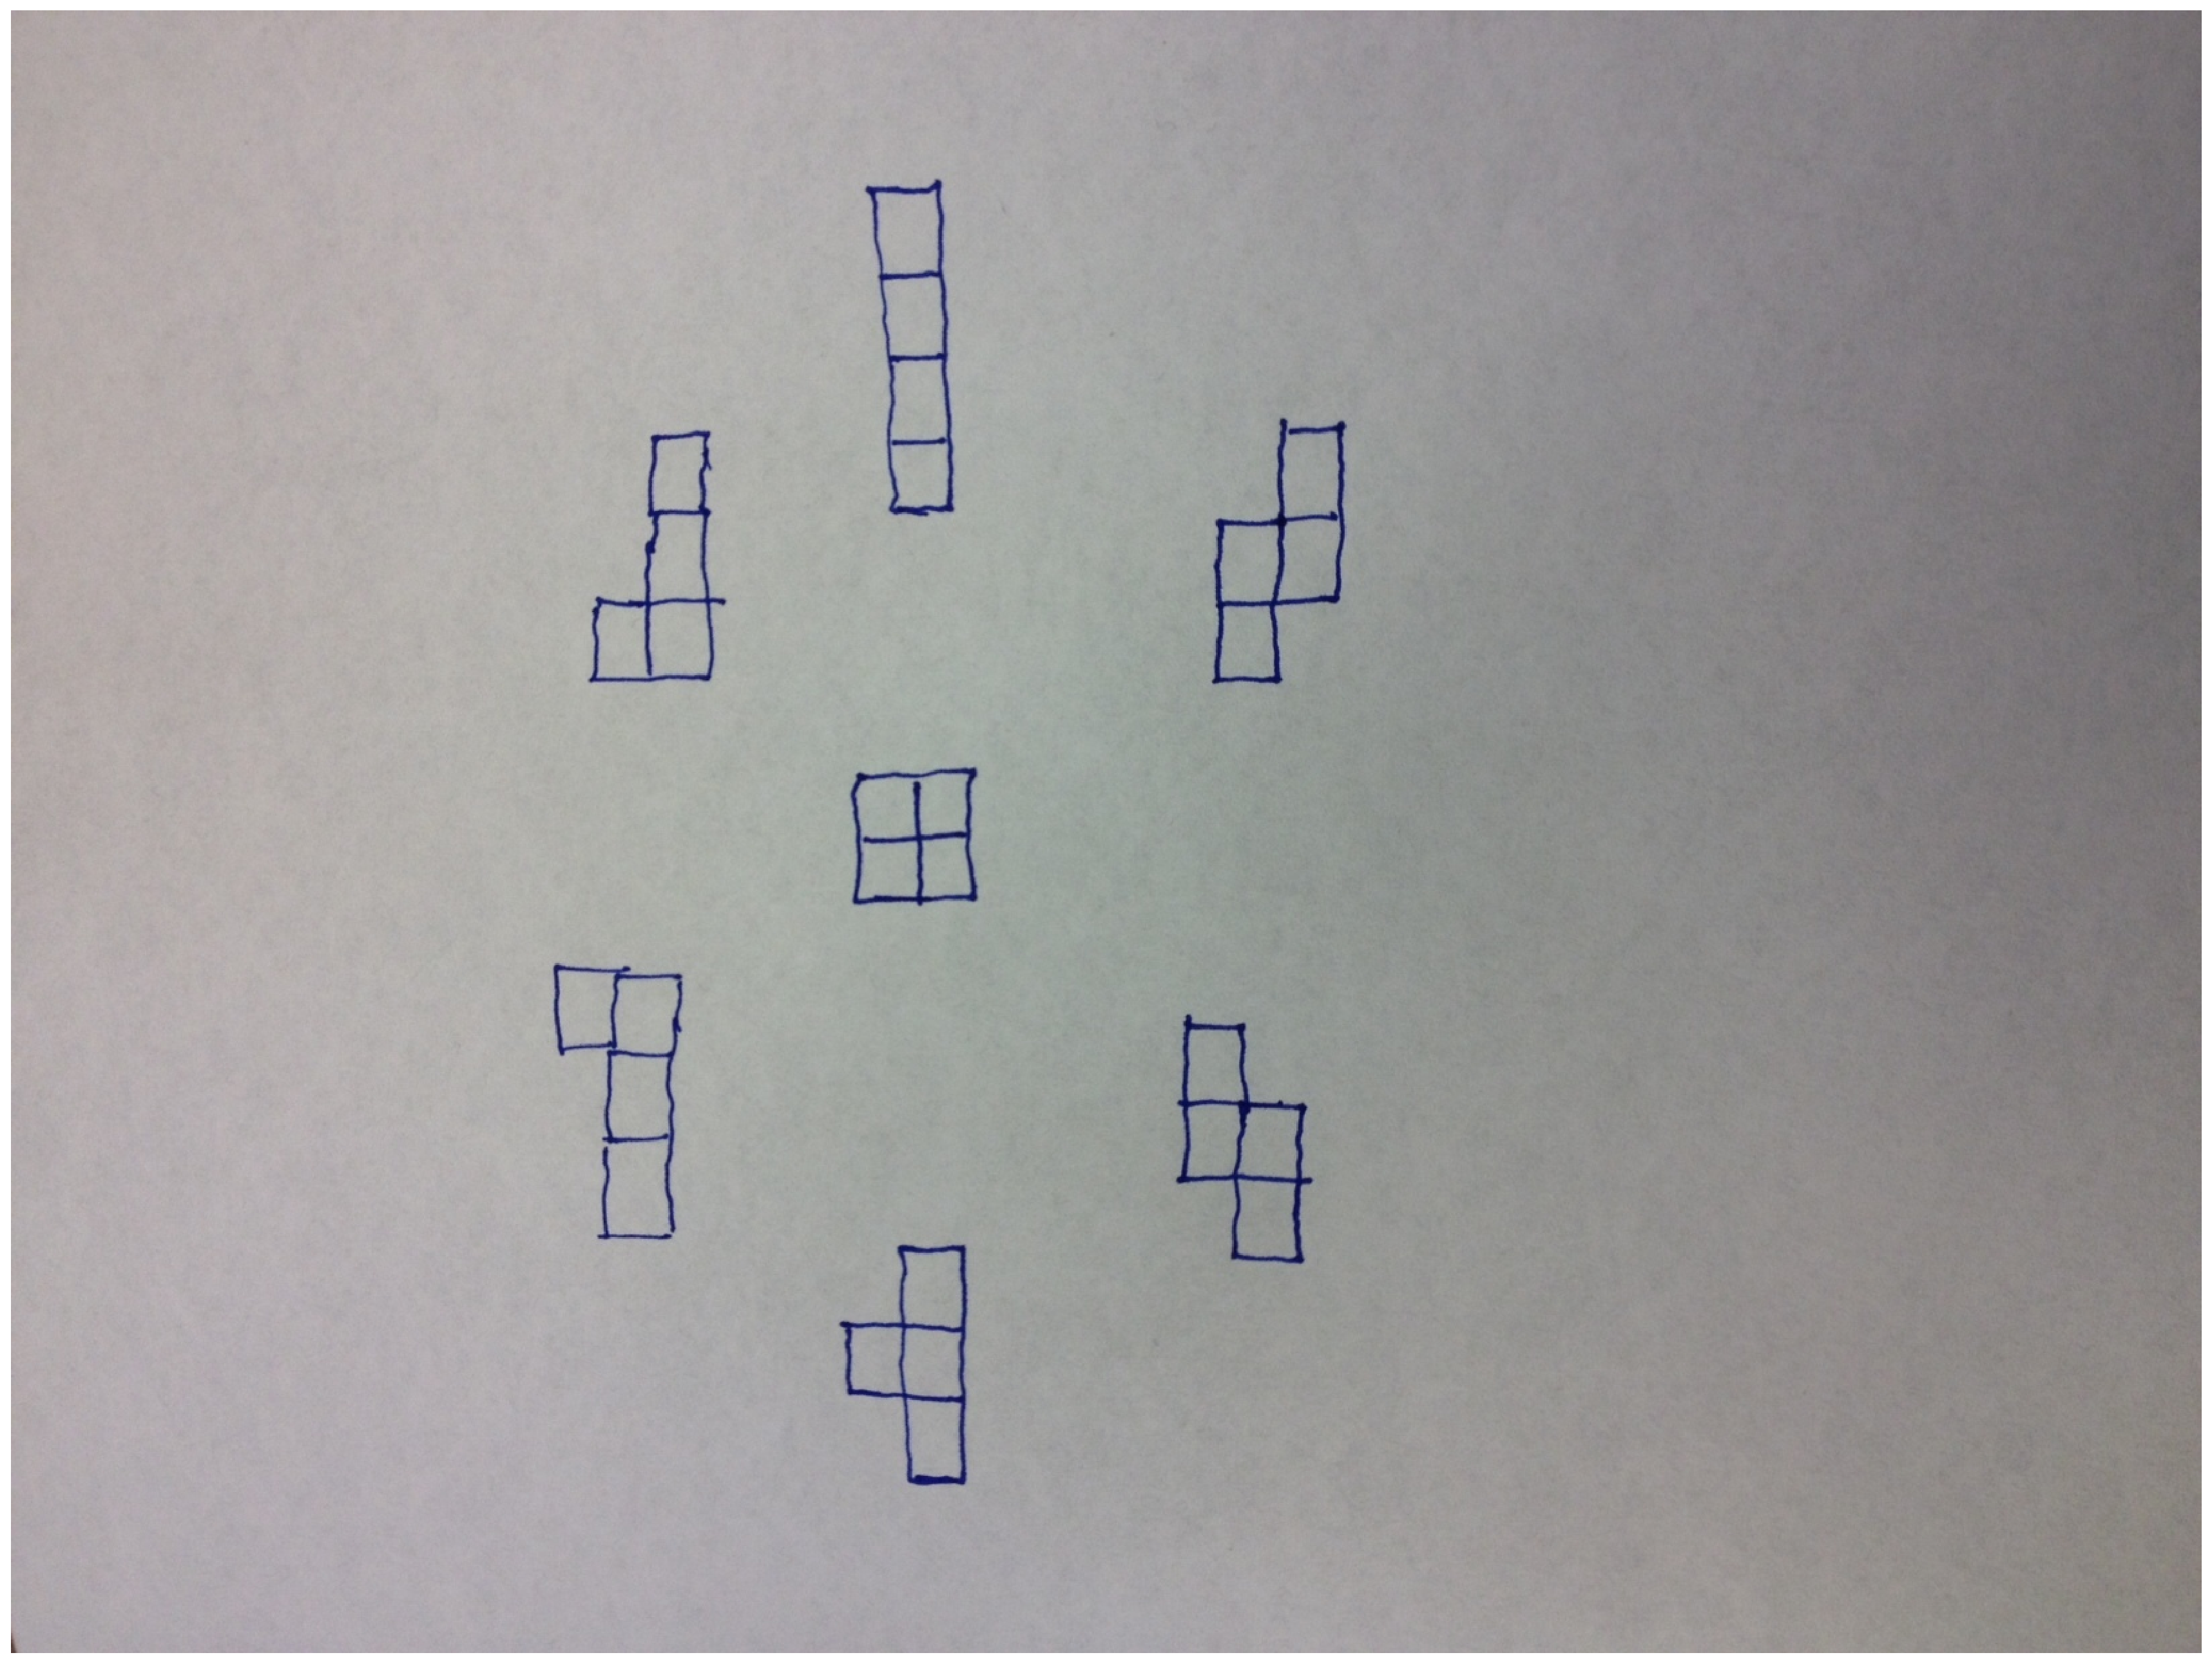
\includegraphics[scale=0.1, angle=0]{tetris.eps}
\caption{The relation between number of faces and connections in the Building Game combinatorial configuration space.}
\label{fig:FacCon}
\end{figure}

\begin{figure}[ht]
  %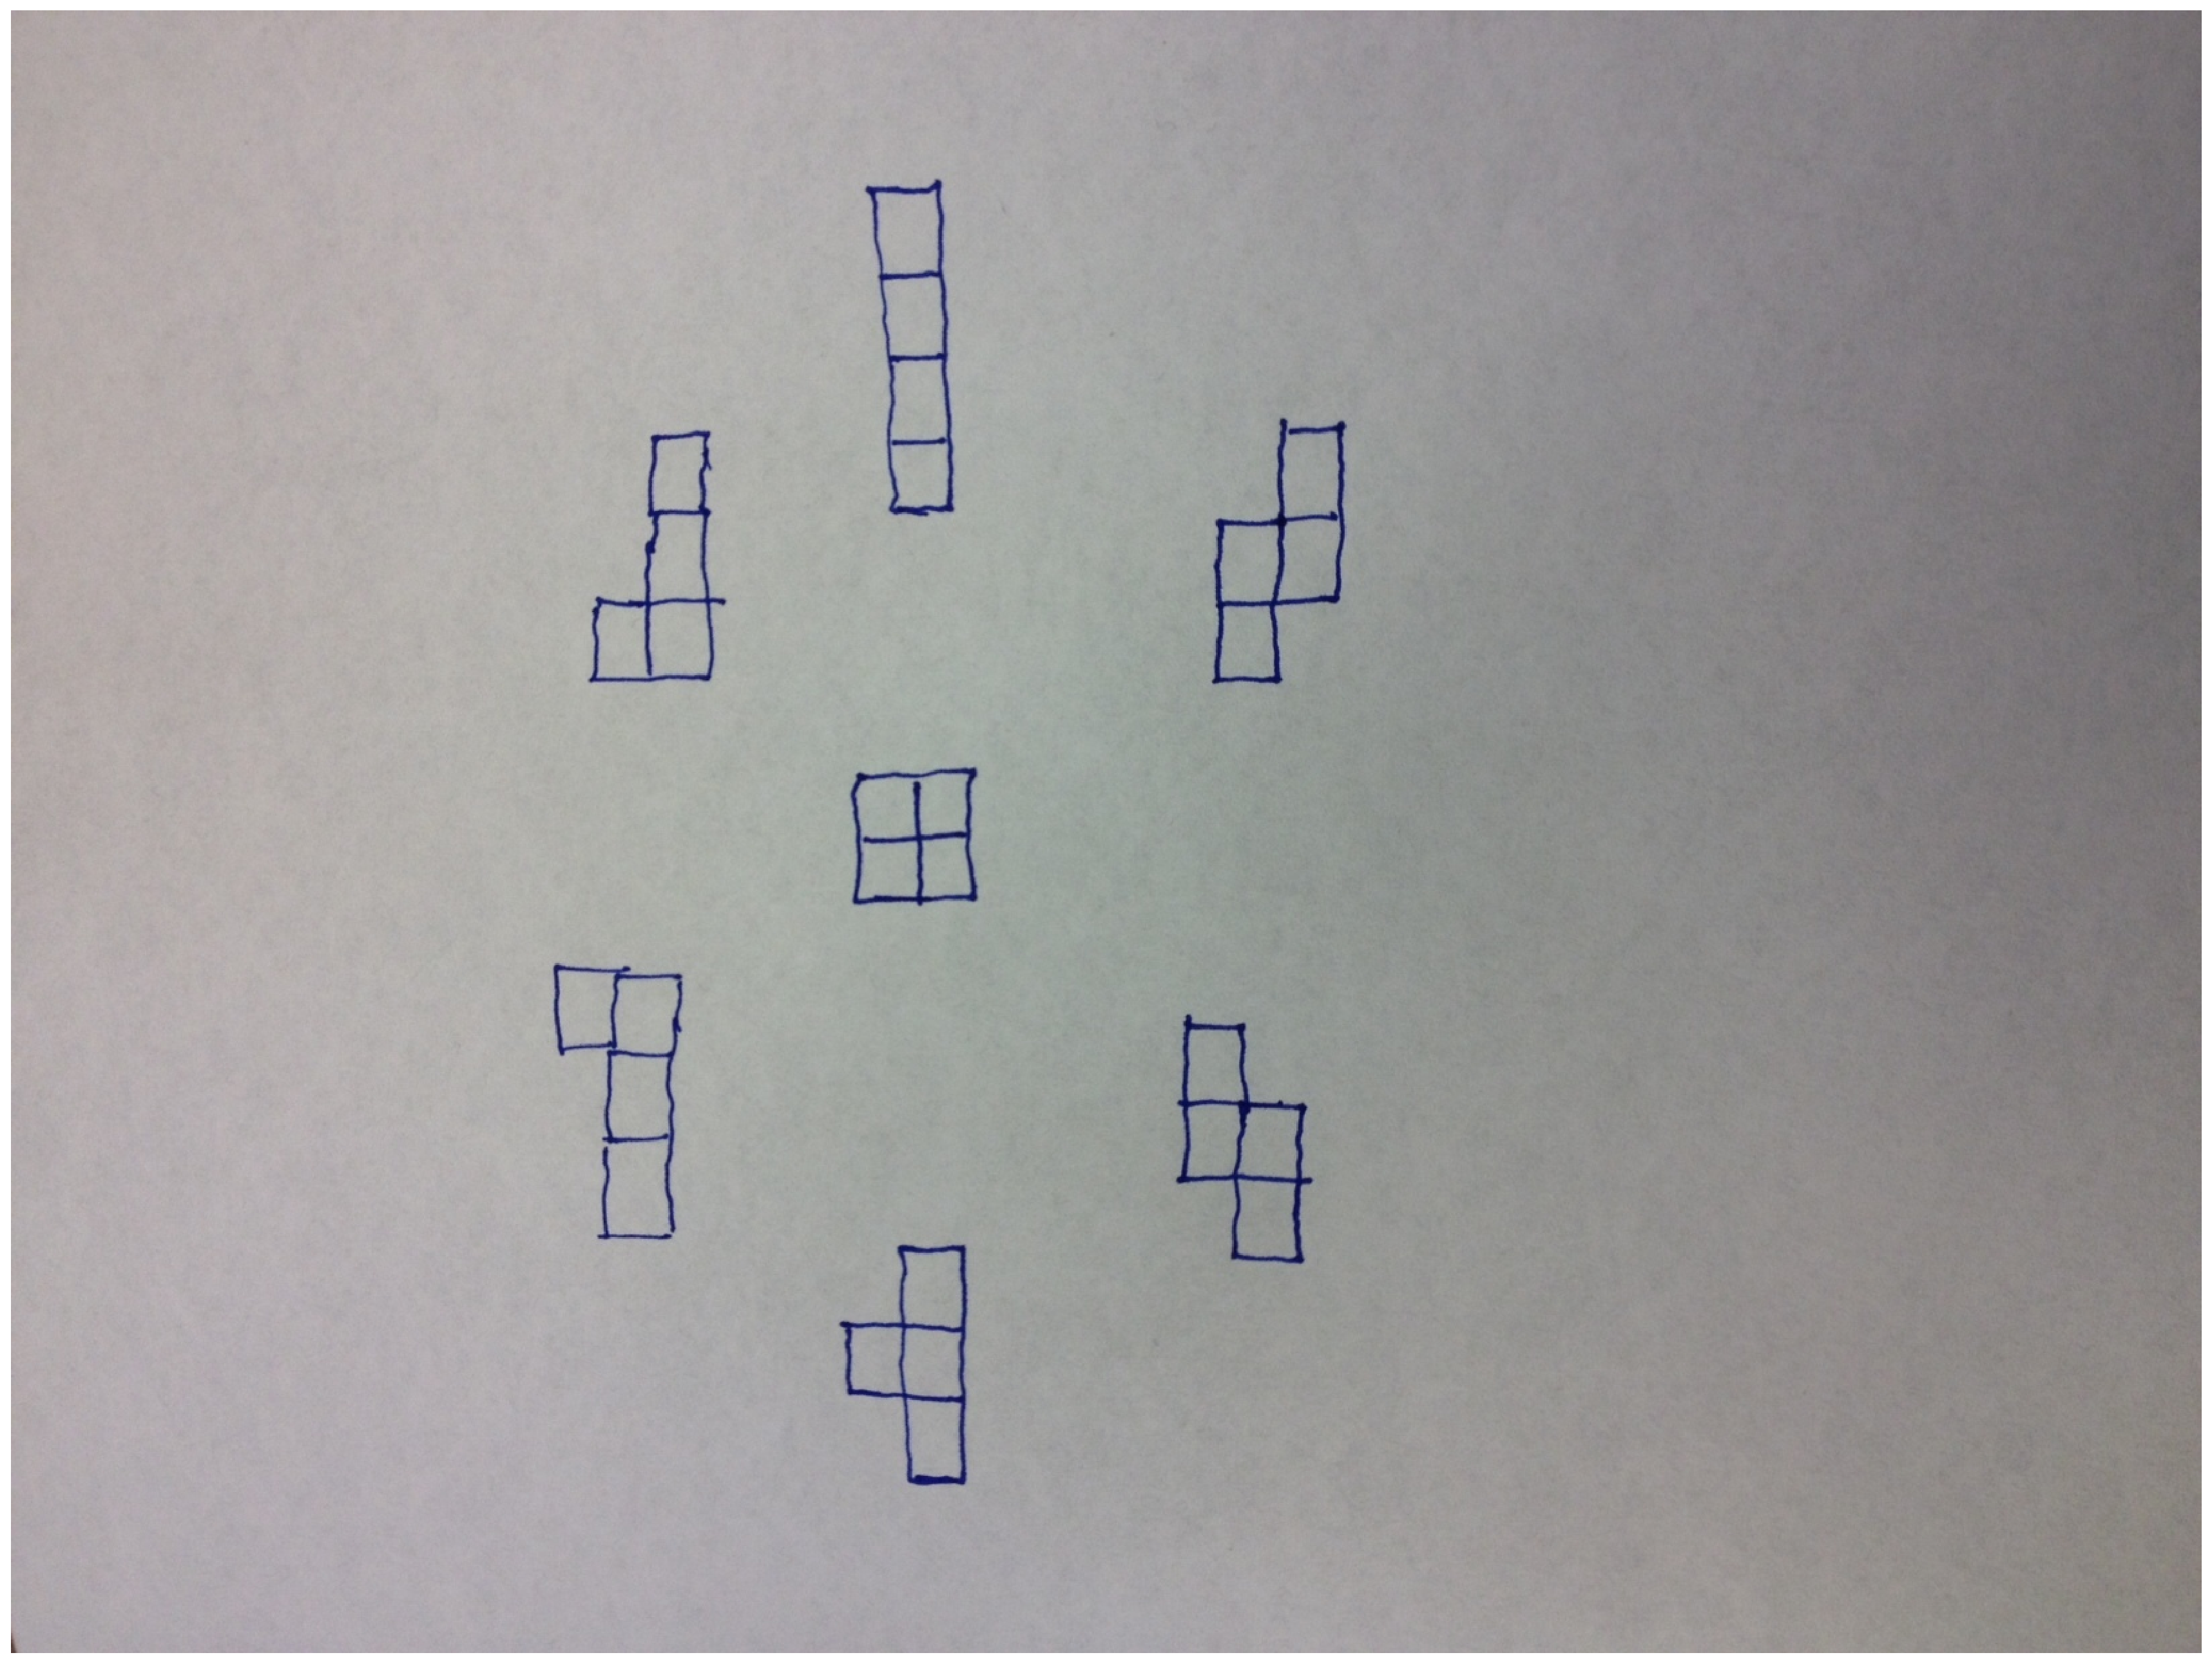
\includegraphics[scale=0.1, angle=0]{tetris.eps}
\caption{The relation between number of faces and paths in the Building Game combinatorial configuration space.}
\label{fig:FacPath}
\end{figure}



\subsection{Shellability}
The theory of polytopes provides a mathematical method for constructing a polytope called a \textit{shelling}. The process, similar to the building game, involves sequentially adding facets of the polytope until all of the facets are added. However, the rules as to which facets may be added at each step of the process is are a bit more restrictive. Ziegler provides the following definitions of a shelling and a shellable polytopal complex CITE. 
\begin{mydef}
\label{def:shelling}
Let $\mathcal{C}$ be a pure $k$-dimensional polytopal complex $\mathcal{C}$. A \textbf{shelling} of $\mathcal{C}$ is a linear ordering $F_1,F_2,\dots,F_s$ of the facets of $\mathcal{C}$ such that either $\mathcal{C}$ is $0$-dimensional (and thus the facets are points), or it satisfies the following conditions:
\begin{enumerate}[(i)]
\item The boundary complex of the first facet $F_1$ has a shelling.
\item For $1 < j \leq s$ the intersection of the facet $F_j$ with the previous facets is non empty and is a beginning segment of a shelling of the $(k-1)$-dimensional boundary complex of $F_j$, that is,
$$F_j \cap \left(\bigcup_{i=1}^{j-1}F_i\right) = G_1 \cup G_2 \cup \cdots \cup G_r$$
for some shelling $G_1, G_2, \dots, G_r, \dots, G_t$ of $\mathcal{C}(\partial F_j)$, and $1 \leq r \leq t$. (In particular, this requires that $F_j \cap (\bigcup_{i=1}^{j-1} F_i)$ has a shelling, so it has to be a pure $(k-1)$-dimensional, and connected for $k > 1$.)
\end{enumerate} 
\end{mydef}

\begin{mydef}
A polytopal complex is \textbf{shellable} if it is pure and has a shelling. 
\end{mydef}

Since we are only concerned with $3$-dimensional polyhedra, the corresponding polytopal complex simply consists of the faces, edges, and verticies of the polyhedron. 

%\begin{mylem}
%The polytopal complex consisting of the verticies of a edge complex is shellable.
%\end{mylem}
%\begin{proof}
%\end{proof}


\begin{mydef}
A Building Game intermediate $x$ is called a \textbf{shellable intermediate} if for every state $x \in [x]$ there is a linear ordering $f_1, f_2, \dots, f_{|x|}$ on the faces of $x$ such that this ordering is a beggining of a shelling $f_1, f_2, \dots, f_{|x|}, \dots f_{||F|}$ of the polytopal complex $F\cup E\cup V$.
\end{mydef}

\begin{mylem}
The polytopal complex consisting of the edges and verticies of a polygonal face is shellable.
\end{mylem}
\begin{proof}
We see that condition $(i)$ from definition~\ref{def:shelling} is satisfied since the boundary complex of each edge is $0$-dimensional.

Condition $(ii)$ is also satisfied since each newly attached edge and the existing partial shelling is a subset of the attached edge's vertices. Since the verticies of the attached edge are $0$-dimensional, any linear order of its verticies is a shelling.
\end{proof}


%\begin{mythm}
%The poly  
%\end{mythm}

\begin{mydef}
A Building Game connection is said to be a \textbf{shellable connection} if the two connected intermediates are both shellable and a Building Game pathway is said to be a \textbf{shellable pathway} if each of its intermediates are shelllable.
\end{mydef}

Figures~\ref{tab:bgePlatShell}, ~\ref{tab:bgeArchShell} and ~\ref{tab:bgeCatShell} detail the shellability statistic for the Platonic, Archimedean, and Catalan solids classes. Because of the added shellability restriction, these count statistics are lower than in the general case, but the combinatorial growth as the number of faces increases is similar.  

%\begin{mylem}
%A shelling order cannot be fixed by a polyhedral rotation. 
%\end{mylem}
%\begin{proof}
%\end{proof}

\begin{figure}[ht]
%\scalebox{0.6}{
\centering
%\textbf{Building Game Enumerative Results for the Platonic Solids}
\begin{tabular}{ l | c | r | r | r}
Polyhedra Name & $|F|$ & Intermediates & Connections & Pathways \\
  \hline    
Tetrahedron                     & 4     & 4     & 5 		& 1\\
Cube                            & 6     & 7     & 7 		& 2\\
Octahedron                      & 8     & 11    & 13 		& 4 \\
Dodecahedron                    & 12    & 52    & 155 		& 2,166\\
Icosahedron                     & 20    & 469   & 1,985 	& 105,999,738\\
\end{tabular}
%}
\caption{Building game enumerative shellability results for the Platonic solids.}
\label{tab:bgePlatShell}
\end{figure}

\begin{figure}[ht]
%\scalebox{0.6}{
\centering
%\textbf{Building Game Enumerative Results for the Platonic Solids}
\begin{tabular}{ l | c | r | r | r}
Polyhedra Name & $|F|$ & Intermediates & Connections & Pathways \\
  \hline    
Truncated Tetrahedron           & 8     & 21		& 40 		& 174\\
Cuboctahedron                   & 14	& 136		& 468 		& 477,776\\
Truncated Cube                  & 14	& 247		& 1,000 	& 5,232,294\\
Truncated Octahedron            & 14	& 342		& 1,464 	& 5,704,138\\
Rhombicuboctahedron             & 26	& 70,887	& 462,721 	& 64,308,526,503,247,584\\
Truncated Cuboctahedron         & 26	& 515,335	& 4,070,813	& 13,890,723,216,176,694,816\\
%Icosidodecahedron               & 32	& ?	& ? 		& ?\\
%Truncated Dodecahedron          & 32	& ?	& ? 		& ?\\
%Truncated Icosahedron           & 32	& ?	& ? 		& ?\\
\end{tabular}
%}
\caption{Building game enumerative shellability results for the Archimedean solids.}
\label{tab:bgeArchShell}
\end{figure}

\begin{figure}[ht]
%\scalebox{0.6}{
\centering
%\textbf{Building Game Enumerative Results for the Platonic Solids}
\begin{tabular}{ l | c | r | r | r}
Polyhedra Name & $|F|$ & Intermediates & Connections & Pathways \\
  \hline    
Triakis Tetrahedron             & 12    & 48		& 115 		& 5,012\\
Rhombic Dodecahedron            & 12 	& 67		& 195 		& 6,258\\
Triakis Octahedron              & 24	& 1,021		& 4,237 	& 210,459,770,300\\
Tetrakis Hexahedron             & 24	& 4,224		& 21,125 	& 5,894,431,702,846\\
Deltoidal Icositetrahedron      & 24	& 33,046	& 208,317 	& 703,619,122,996,096\\
Pentagonal Icositetrahedron     & 24	& 95,326	& 657,013 	& 7,572,459,719,248,765\\
Rhombic Triacontahedron         & 30	& 97,741	& 702,219 	& 7,057,239,571,753,327,764\\
\end{tabular}
%}
\caption{Building game enumerative shellability results for the Catalan solids.}
\label{tab:bgeCatShell}
\end{figure}

\begin{figure}[ht]
  %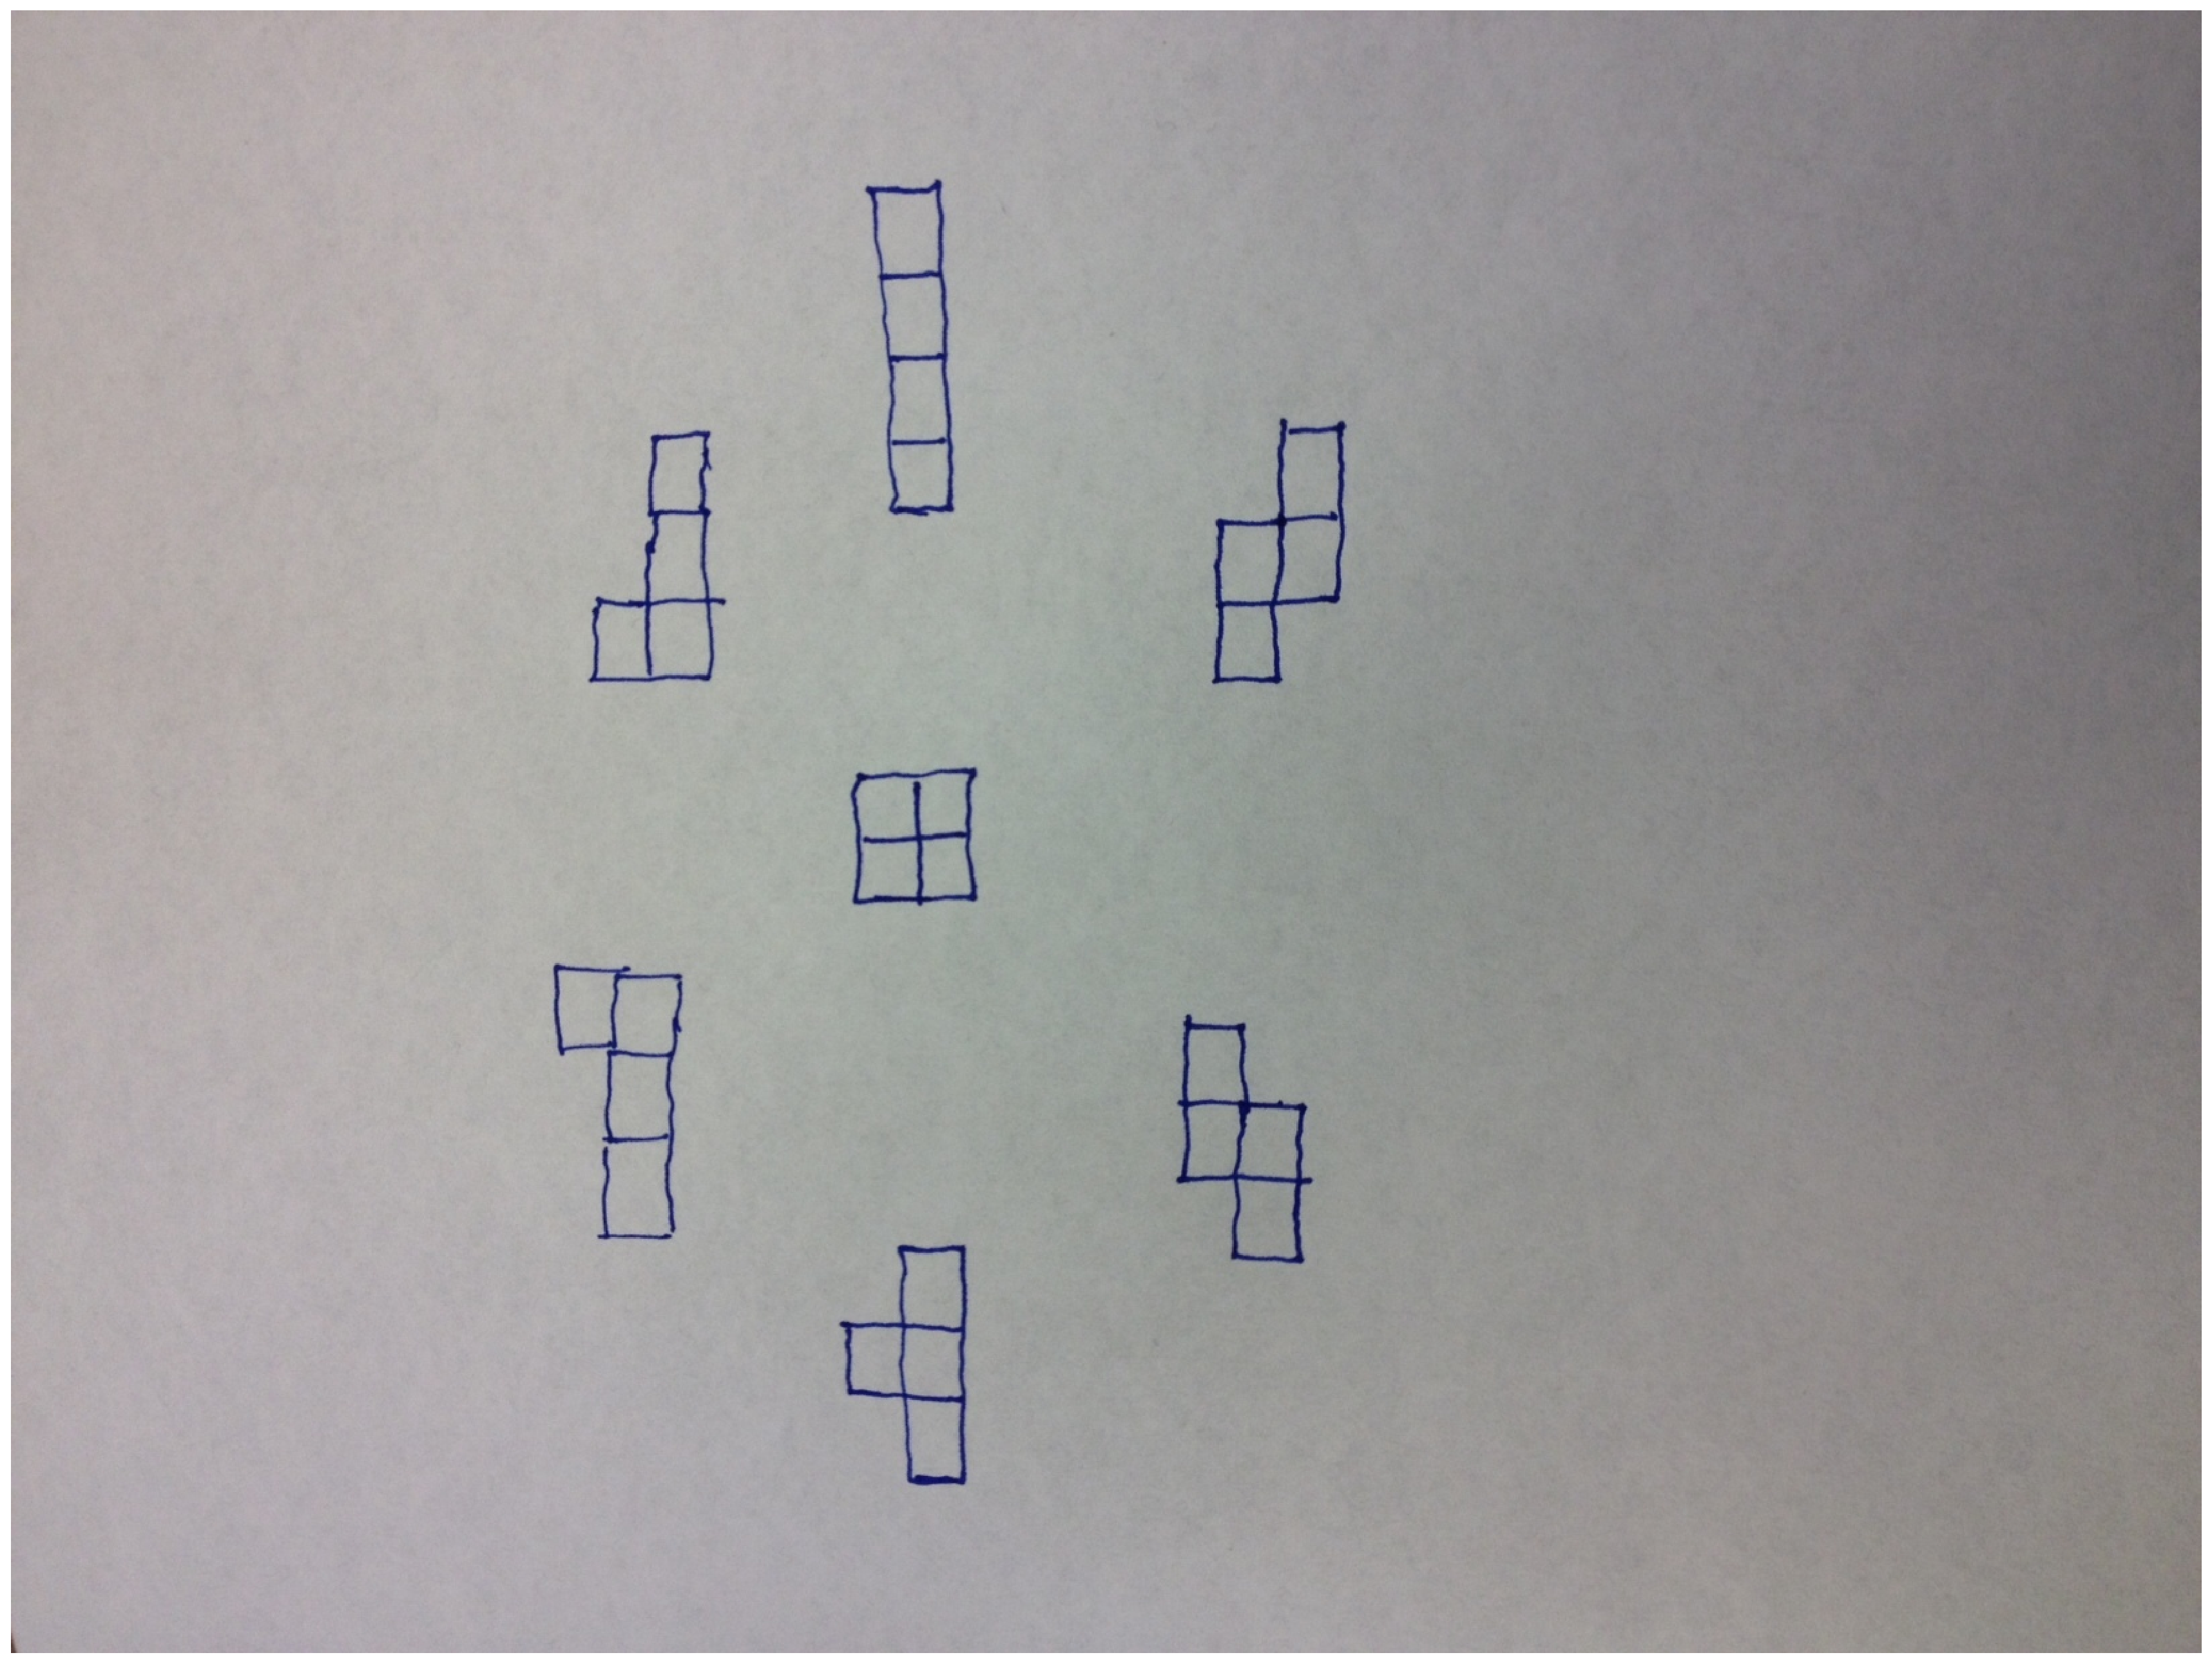
\includegraphics[scale=0.1, angle=0]{tetris.eps}
\caption{The relation between number of faces and shellable intermediates in the Building Game combinatorial configuration space.}
\label{fig:FacIntShell}
\end{figure}

\begin{figure}[ht]
  %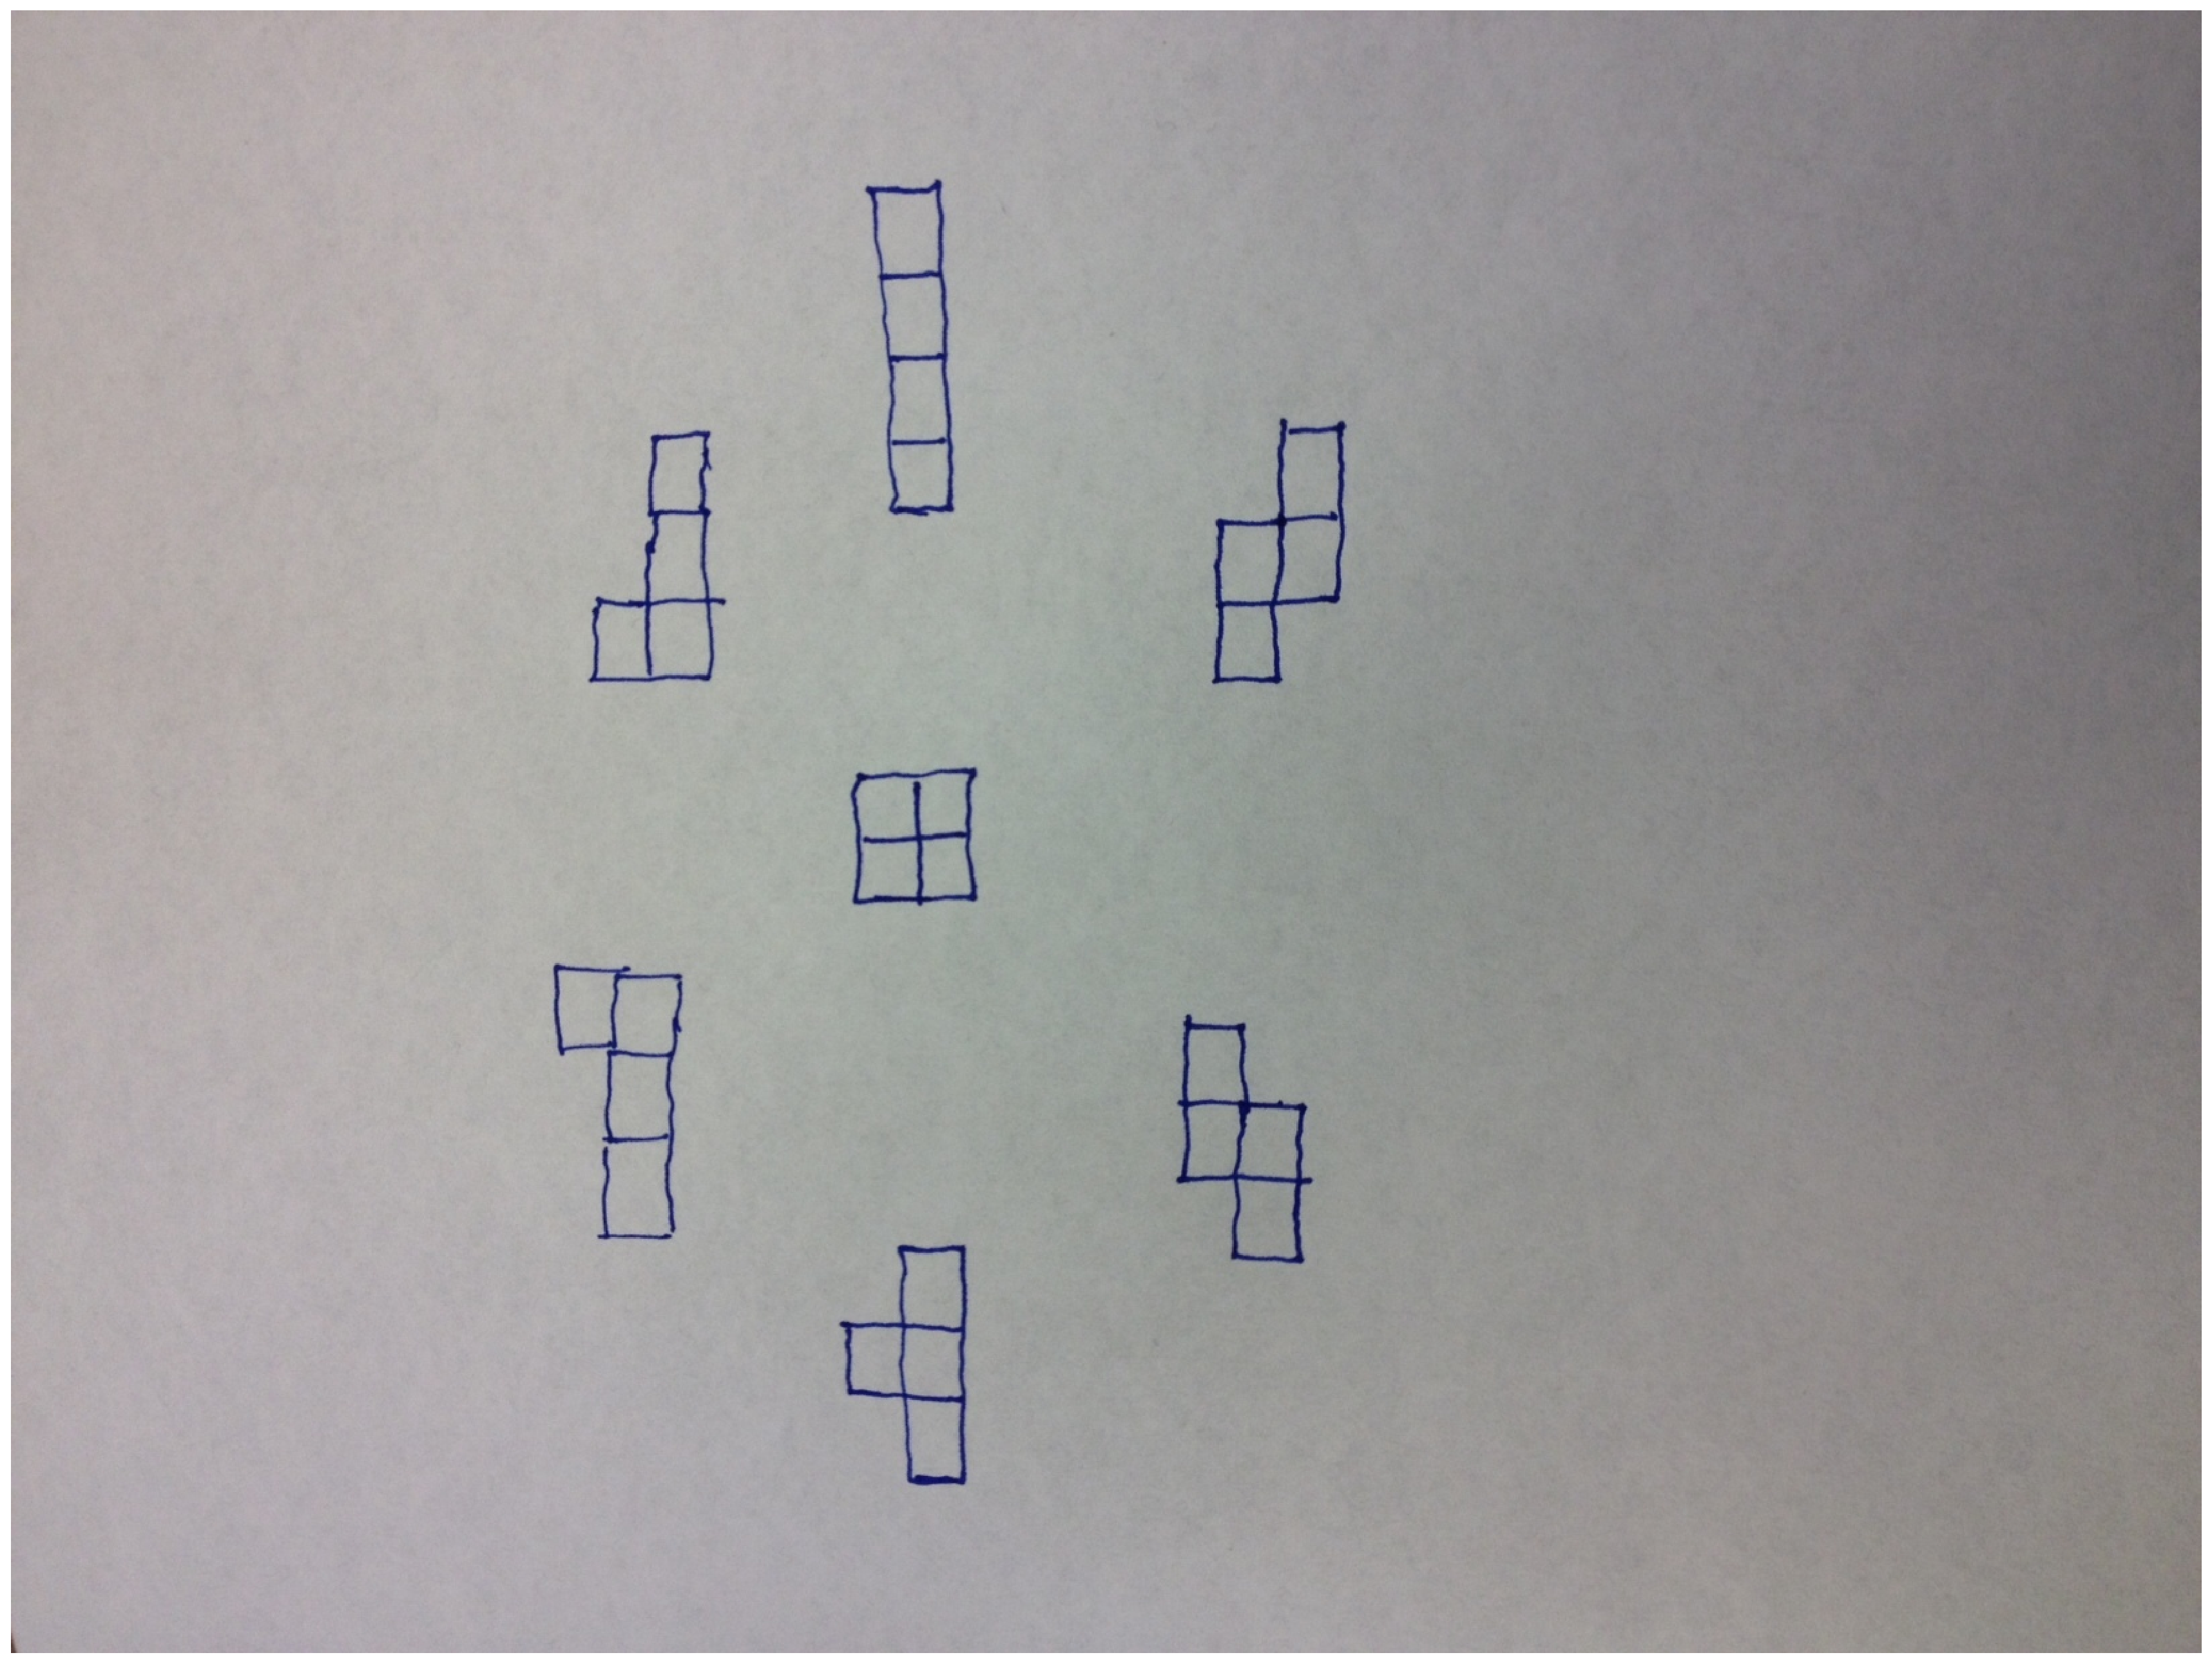
\includegraphics[scale=0.1, angle=0]{tetris.eps}
\caption{The relation between number of faces andc shellable connections in the Building Game combinatorial configuration space.}
\label{fig:FacConShell}
\end{figure}

\begin{figure}[ht]
  %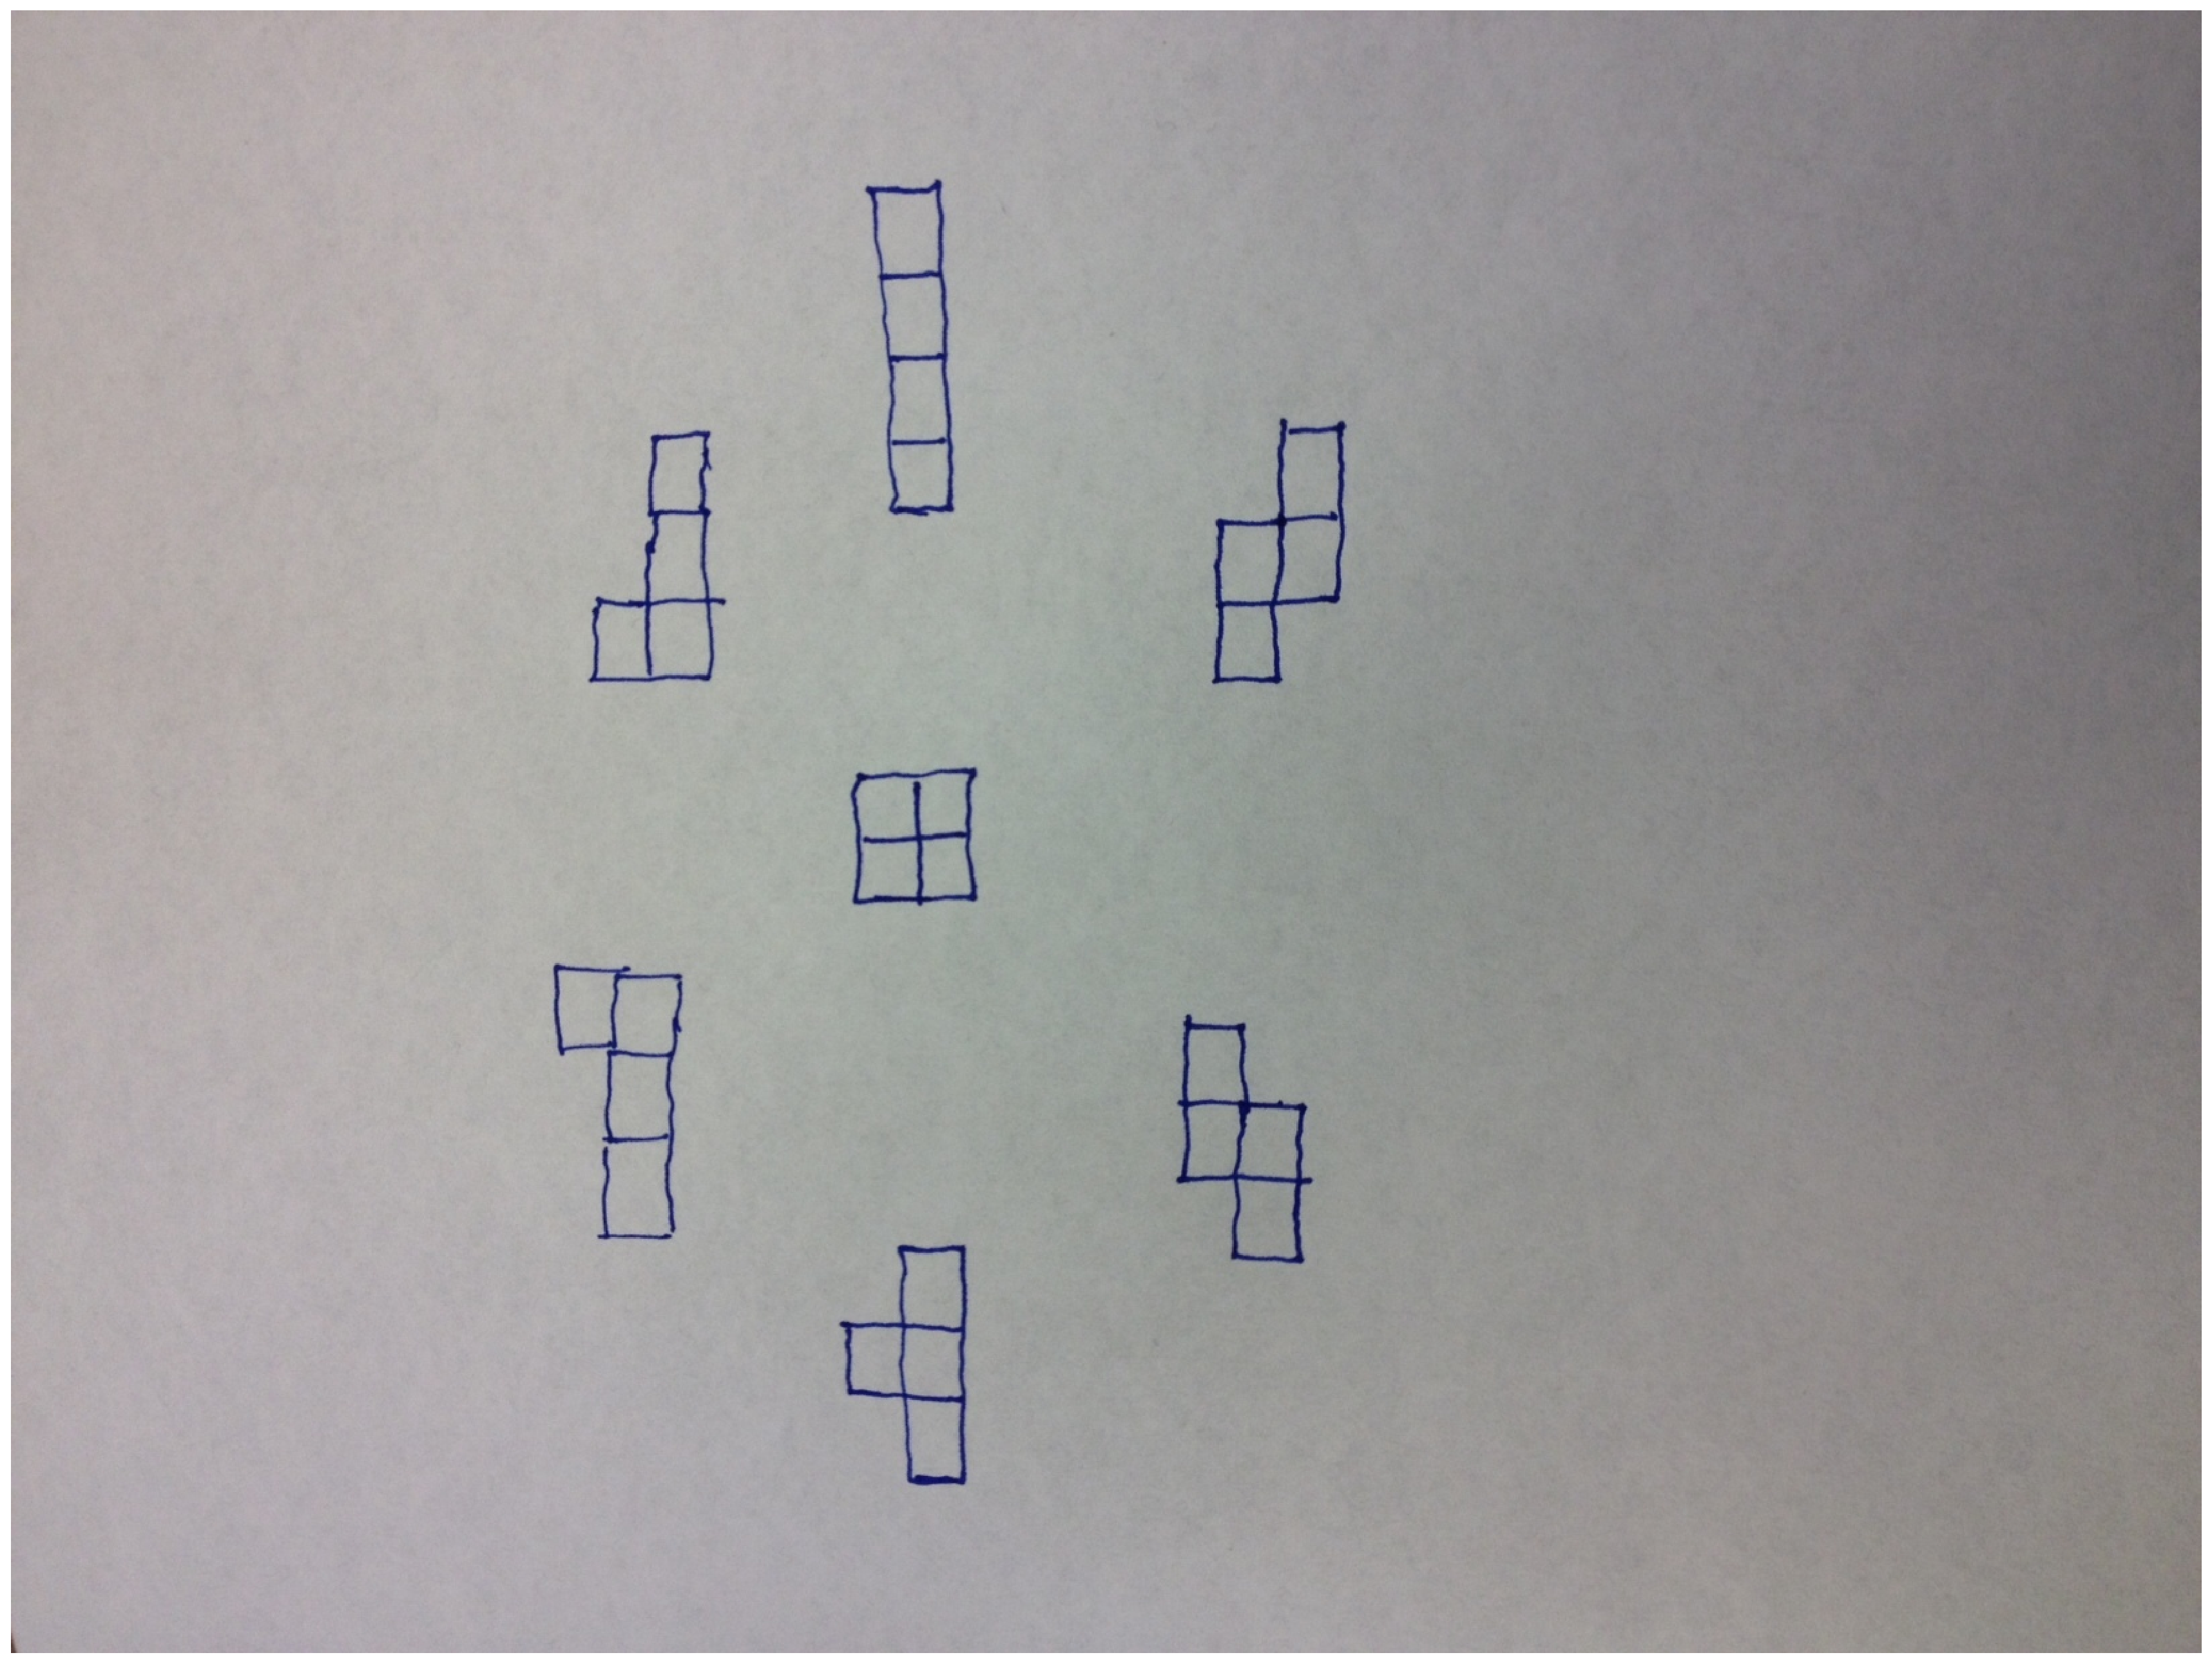
\includegraphics[scale=0.1, angle=0]{tetris.eps}
\caption{The relation between number of faces and shellable paths in the Building Game combinatorial configuration space.}
\label{fig:FacPathShell}
\end{figure}

\subsection{Shelling Enumeration}

To our knowledge, the enumeration of the number of shellings of the polyhedra in the Platonic, Archimedean, and Catalan solid classes remaints an open problem. Here we present these enumerations for the polyhedra of up to $30$ faces.The concept of a shelling is similar to to that of a pathway. Using the structure of each computed combinatorial configuration space, a method for counting the number of shellings of a polyhedron is derived.

\begin{mythm}
The total number of shellings for a polyhedral complex generated by a polyhedron is the number of shellable building game pathways times the order of the rotation group of the polyhedron. 
\begin{align}
\#\{shl\} &= \sum_{p \in \{shell paths\}}|[x^{p_1}]|\prod_j^{|F|-1}S_{p_jp_{(j+1)}} 
\end{align}
\end{mythm}
\begin{proof}
Show each degeneracy of each pathway produces a unique shelling. And then that any rotation of each of these shellings is also unique.
\begin{align}
\#\{shl\} &= \sum_{f_1 \in F} \mathbbm{1}_{sh(\emptyset,f_1)} \cdots\sum_{f_k \in F\setminus \{f_1,\dots,f_{k-1}\}} \mathbbm{1}_{sh(\{f_1,\dots,f_{k-1}\}, f_k)}\cdots \sum_{f_{|F|} \in F\setminus \{f_1, f_2, \dots, f_{|F|-1}\}}\mathbbm{1}_{sh(\{f_1, f_2, \dots, f_{|F|-1}\},f_{|F|})}  \\
&= \sum_{f_1 \in F} \mathbbm{1}_{sh(\emptyset,f_1)} \cdots\sum_{f_k \in F\setminus \{f_1,\dots,f_{k-1}\}} \mathbbm{1}_{sh(\{f_1,\dots,f_{k-1}\}, f_k)}\cdots \sum_{x^{p_{|F|}}: [x^{p_{|F|-1}}] \xrightarrow{shell} [x^{p_{|F|}}]} S_{p_{|F|-1}p_{|F|}}  \\
&= \sum_{f_1 \in F} \sum_{x^{p_2}: [x^{p_1}] \xrightarrow{shell} [x^{p_2}]} S_{p_{1}p_{2}}  \cdots \sum_{x^{p_{|F|}}: [x^{p_{|F|-1}}] \xrightarrow{shell} [x^{p_{|F|}}]} S_{p_{|F|-1}p_{|F|}}  \\
&= \sum_{[x^{p_1}} |[x^{p_1}]| \sum_{x^{p_2}: [x^{p_1}] \xrightarrow{shell} [x^{p_2}]} S_{p_{1}p_{2}}  \cdots \sum_{x^{p_{|F|}}: [x^{p_{|F|-1}}] \xrightarrow{shell} [x^{p_{|F|}}]} S_{p_{|F|-1}p_{|F|}}  \\
&= \sum_{p \in \{shell paths\}}|[x^{p_1}]|\prod_j^{|F|-1}S_{p_jp_{(j+1)}} 
\end{align}
\end{proof}

Using dynamic programming we can compute the number of shellings explicitly without having to explicitly consider each pathway individually. Define the quantity $a_{ik}$ as follows.
\begin{align}
a_{i,k} &\doteq  \sum_{\substack{\text{shellable subpaths}:\\ p_1, \dots, p_k \\ x^{p_k} \in [x^i]}}|G.x^{p_1}|\prod_{j=1}^{k-1}S_{p_j p_{j+1}} \end{align}
Using this definition, we first not that the number of shellings, which is the quantity of interest, is equal to $a_{N,|F|}$ where $x^N = F$. Now, we set up the following recursion that will be the basis for our computation. 
\begin{align}
a_{i,k} &\doteq \sum_{\substack{\text{shellable subpaths}:\\ p_1, \dots, p_k \\ x^{p_k} \in [x^i]}}|G.x^{p_1}|\prod_{j=1}^{k-1}S_{p_j p_{j+1}} \\  
&= \sum_{[x^\ell]:[x^\ell]\xrightarrow{shell}[x^i]} \sum_{\substack{\text{shellable subpaths}:\\ p_1, \dots, p_{k-1} \\ x^{p_{k-1}} \in [x^\ell]}}|G.x^{p_1}|S_{\ell i}\prod_{j=1}^{k-2}S_{p_j p_{j+1}} \\
&= \sum_{[x^\ell]:[x^\ell]\xrightarrow{shell}[x^i]} S_{\ell i} \sum_{\substack{\text{shellable subpaths}:\\ p_1, \dots, p_{k-1} \\ x^{p_{k-1}} \in [x^\ell]}}|G.x^{p_1}|\prod_{j=1}^{k-2}S_{p_j p_{j+1}} \\
&= \sum_{[x^\ell]:[x^\ell]\xrightarrow{shell}[x^i]} S_{\ell i} a_{\ell, k-1}
\end{align}
Thus, using the base cases $a_{j,1} = |G.x^j|$ for each single faced intermediate $[x^j]$, we can use this relation to recursively solve for the number of shellings $a_{N,|F|}$.



\subsection{Bounds and Asymptotics}
There is a clear relation between the number of faces in a polyhedron and then number of intermediates it has. However, that relationship also greatly depends on the polyhedral symmetry group. For instance, if you have a polyhedron with a small number of faces and a trivial rotation group consisting only of the identity, every edge-connected subset of the polyhedron's faces will be a distinct intermediate. In agregate, this may mean that the polyhedron has more intermediates than another polyhedron with more faces, yet a larger symmetry group. 

An upper bound on the number of intermediates is possible using the theory of group actions. Consider the set of all subsets $2^F$ of a polyhedron with rotation group $G$. Trivially $|2^F/G|$ is an upper bound on the number of intermediates since it simply relaxes the connectivity requirement for a subset to be a building game state. Using Burnside's lemma, we see that 
\begin{align}
  \label{eq:IntUB}
  |2^F/G| &= \frac{1}{|G|}\sum_{g \in G}|(2^F)^g| \\
  &> \frac{|(2^F)^e|}{|G|} \\
  &= \frac{|2^F|}{|G|} \\
  &= \frac{2^{|F|}}{|G|}
\end{align}
which is not a particularly good bound in practice. The exact value of $|2^F/G|$ is calcuable with minimal computer assistance. For the cube, the bound is fairly tight, only including the two non-intermediates corresponding to the empty subset of faces, and the non-connected subset consisting of the top and bottom faces. Thus the cube has the bound $|2^F/G| = 10 \geq 8$. In the case of the tetrahedron, the only overcounted subset of faces is the empty one and the bound is $|2^F/G| = 5 \geq 4$. However, in the case of the icosahedron we have $|2^F/G| \geq \frac{2^{20}}{60} \approx 17476.3 \gg 2649$. Here we use the approximate bound $\frac{2^{|F|}}{|G|}$ which is the largely dominant term in the sum from equation~\ref{eq:IntUB}.

We can get a similar bound on the number of intermediates with a particular number of faces,
\begin{align}
  |\{x \in 2^F: |x| = k\} /G| &= \frac{1}{|G|}\sum_{g \in G}|\{x \in 2^F: |x| = k\}^g| \\
  &> \frac{|\{x \in 2^F: |x| = k\}^e|}{|G|} \\
  &= \frac{|\{x \in 2^F: |x| = k\}|}{|G|} \\
  &= \frac{{|F| \choose k}}{|G|}
\end{align}
but again, this is not particularly useful, especially for intermediates with $\sim\frac{|F|}{2}$ faces.

Since the building game is similar in spirit to polyomino enumeration, one might try to assimilate some the techniques used for polyominos. For example, through fairly simple arguments, one can show that $s_ms_n \leq s_{m+n}$ where $s_m$ is the number of unique polyominos with $m$ subunits CITE. This leads to the bound $s_m \leq (const)^m$. Trying to set up such a relation in the building game is sounds initially appealing, but there is a fundamental diefference between the two growth models that makes this approach futile. In the polyomino case, there is no limit to the number of subunits that can be considered. Importantly, this is not the case for the bulding game since an intermediate can only have $|F|$ faces at most. Thus any such reccurrence relation for the building game will result in a good upper bound for the intermediates with a small number of faces at best.

The formulation of meaningful bounds for the number of building game intermediates with $k$ faces remains an open problem, especially for $k \sim \frac{1}{2}|F|$. At the root of the problem is the difficulty in mathematicallly describing the subsets of $F$ are edge connected. Future approches may incorperate enumeration results for connected subgraphs or Hamiltonian paths since these topics explicitly acknowledge connectedness properties. 

From looking at the statistics on number of faces $|F|$ of a polyhedron and the number of intermediates in its commbintorial configuration space, it is natural to want to make statements about the asymptotic growth of thr combinatorial configuration space's size. Unfortunately, when formed in this way, the problem is ill-posed. To discuss assymptotics, we must first specify an infinite class of polyhedra. The Platonic, Archimedean, and Catalan Solid classes that we've worked with thus far are all finite though, so other choices must be consider. One option is to take an existing polyhedron in one of these classes and create an infinite family by describing finer and finer tiling on top of the polyhedron's faces. If designed cafefully each member of the tiled polyhedron family will have the same symmetry group, even as the number of faces grows. 

Similar to polyhedra with tiled faces are the icosahedron viral capsids indexed by T-number. This number is related to the number of protein subunits in the virust. When each subunit is idealized as a polygon, a T-capsid will consist of $12$ pentagons and $10(T-1)$ hexagons. Interestingly, this makes most of the icosahedral viral capsid equivalent to the dual of an icosahedron with each face consisting of $T$ trianglular tiles. This would certainly be an interesting an relevant familty of polyhedra to consider, though we leave it as an opn problem.

\section{Computational Methods}

To compute the combinatorial configuration space and enumerate the intermediates for a particular polyhedron, we use a brute force method. Computation begins with first enumerating the intermediates with a single face. This enumeration is then used to compute the intermediates with two faces. This process proceeds iteratively until all intermediates are accounted for. Figure~\ref{alg:CCS} outlines the detailed algorithm for this computation. 

At each stage of our algorith, we know the set of intermedites that have $k$ faces, which we call $A_k$, and use this information to compute the set of faces with $k+1$ faces, $A_{k+1}$. Since all intermediates in $A_{k+1}$ must be formed by adding a single face to an intermediate from $A_k$, we take each intermediate $[x] \in A_k$ and try adding each face to $x$ that is allowable under the building game rules. This means we look at every face $f \in F$ and check if $f \not\in x$ and also that $x$ is edge connected to a face $\hat{f}$ that is in $x$. For every such faces $f$, we look at the new $(k+1)$-faced state $y \doteq x\cup \{f\}$. Since we know that $[y]$ is a building game intermediate, it must be represented in $A_{k+1}$, however before adding $y$ to $A_{k+1}$, we must verify that there is no $\hat{y}$ already in $A_{k+1}$ such that $y \in [\hat{y}]$.

\begin{figure}[ht]
\centering
\begin{algorithmic}
  \State $A_1\gets \{\{f\} : f \in F\}$ 
  \For{$\{f\} \in A_1$}
  \If{$\exists \{\hat{f}\} \in A_1 \setminus \{f\} : [\{\hat{f}\}\ ]= [\{f\}]$}
  \State $A_1 \gets A_1 \setminus \{\{f\}\}$
  \EndIf
  \EndFor
  \State $A_2, \dots, A_{|F|} \gets \{\}$ 
  \For{$k = 0,\dots,|F|-1$}
  \For{$x \in A_k$ }
  \For{$f \in F\setminus x$ such that $\exists \hat{f} \in x$ with $f$ and $\hat{f}$ sharing an edge. }
  \State NewIntermediate $\gets True$
  \For{$\hat{y} \in A_{k+1}$}
  \If{$y \in [\hat{y}]$}
  \State NewIntermediate $\gets False$
  \State Add connection $[x] \leftrightarrow [\hat{y}]$ to combinatorial configuration space.
  \EndIf
  \EndFor
  \If{NewIntermediate $= True$}
  \State $A_{k+1} \gets A_{k+1} \cup \{y\}$
  \State Add connection $[x] \leftrightarrow [y]$ to combinatorial configuration space.
  \EndIf
  \EndFor
  \EndFor
  \EndFor
\end{algorithmic}
\caption{Algorithm for interatively enumerating the Building Game combinatorial configuration space.}
\label{alg:CCS}
\end{figure}

The act of comparing two states $y$ and $\hat{y}$ to check if they are members of the same intrmediate is the task where the majority of computational time is spent. The brute force method of checking if $y \sim \hat{y}$ involves checking if $g.y = \hat{y}$ for each $g \in G$. If a $g$ is found that makes this equality hold, then $[y] = [ \hat{y}]$ and the computation terminates and we know that $[y]$ is not a new intermediate. In this case, nothing is added to $A_{k+1}$ but a connection $x \leftrightarrow \hat{y}$ is added in the combinatorial configuration space. Furthermore, by tracking how many time a particular connection $x \leftrightarrow \hat{y}$ is found, the forward degeneracy numbers can be computed. 

\subsection{Hash Functions}
In practice, we implement a hash function $\textswab{h}$ that maps each state to an integer with the property that if $[y] = [\hat{y}]$, then $\textswab{h}(y) = \textswab{h}(\hat{y})$. If we can design such a function and it is computable in significantly less time relative to the brute force method of trying every rotation, the overall computation can be majorly diminished. 

When checking if two states $y$ and $\hat{y}$ are members of the same intermediate, we first check if $\textswab{h}(y) = \textswab{h}(\hat{y})$. If they do not have the same hash, then they cannot be members of the same intermediate and the check is complete. Alternatively, if they do have identical hashes, it is not a guarentee that they are members of the same intermediate, so the brute force rotation method must be used. If the hash is carefully designed then this false positive rate ($\textswab{h}(y) = \textswab{h}(\hat{y})$ when $[y] \neq [\hat{y}]$) is small and almost all of the brute force calculations will result in a positive match. 

In an ideal world, a hash function that also gives the property $[x] = [\hat{x}]$ whenever $\textswab{h}(x) = \textswab{h}(\hat{x})$ would be best. However we have not been able to find such an $\textswab{h}$ that is computable in a relatively reduced amount of time in comparison to the brute force method. We leave the existance of such a hash as a possibility. 

Since any hash we choose must a function that maps states that are rotations of each other to the same integer, we look at local connectivity properties. For each face $f_k \in F$ define its local connectivity within $y$ as  $\textswab{h}_k(y) = |\{\hat{f} \in F : \hat{f} \in y, f_k \cap \hat{f} \in E\}|$, the number of faces adjacent to $f_k$ that are in $y$. Since this connectivity is preserved by rotations, even though we wont necesarily have $\textswab{h}_k(y) = \textswab{h}_k(\hat{y})$ when $[y] = [\hat{y}]$, if we take a histogram of all values of $\textswab{h}_k$ for $k = 1,\dots,|F|$, the histogram will be the same for both $y$ and $\hat{y}$. Once a histogram is computed, the final hash $\textswab{h}$ is just a simple function that maps histograms to integers.

There are many variants of statistics that this histogram strategy can be used with. We found that taking separate histograms for faces in $y$ and faces not in $y$ provided a hash with less false positives, while only increasing the hash computation time marginally. Depending on the polyhedron, the implementation of this hash lead to an over all speed up of at least an order of magnitude over the purely brute force method.  

\subsection{Data Structures}

Before the computation of the combinatorial configuration space, we hardcode an enumeration $f_1, \dots, f_{|F|}$ of the faces of our polyhedron. Then, any state $x$ is represented by a binary vector of length $|F|$ with a one in the $k$th entry if $f_k \in x$ and zero otherwise. With this convention, each rotation $g \in G$ corresponds to a permutation of the indices of $x$. Each such permutation in the group is precomputed and then applies as necessary when performing a brute force comparison of two states. To track the connectivity structure of the polyhedron, an adjaceny list on faces is stored as a two dimensional array. For each face number, the adjacency list specifies the index of adjacent faces.

Each group of $k$-faced intermediates $A_k$ is stored as a hash table using the previously described hash function. This allows for order one lookup of intermediates already in the $A_k$ that share the hash of a new proposal intermediate. 

\subsection{Run Time}

The computing time required to enumerate the combinatorial configuration space is heavily dependent on the number of intermediates that are found. Since we do not have a tight bound on the number of intermediates as a function of simple statistics of the polhedron (faces, edges, etc.), it is difficult to provide a meaningful estimates on the time required to compute the combinitorial configuration space without explicit knowledge of its size a priori.

That said, we can express an upper bound on the number of state to state comparisons that are required as a function of the intermediate sets $A_1,\dots,A_{|F|}$. 

\begin{align}
\#\text{comparisons} &\leq \sum_{k=1}^{|F|-1} \sum_{x \in A_k} \sum_{f \in F\setminus x} \sum_{\hat{y} \in A_{k+1}} 1 \\
&\leq |F|\sum_{k=1}^{|F|-1}|A_k||A_{k+1}| 
%&\leq |F|\sum_{k=1}^{|F|-1} {|F| \choose k} {|F| \choose k+1}  \\
\end{align}


\subsection{Implementation}
